\documentclass[12pt,titlepage]{article}
\usepackage[noxcolor,notheorems,envcountsect]{beamerarticle}
\usepackage{geometry}
 \geometry{
 a4paper,
 total={170mm,257mm},
 left=20mm,
 top=20mm,
 }
\usepackage[utf8,utf8x]{inputenc}
\usepackage{amsmath,amssymb,amsfonts,booktabs,empheq,lmodern,mathtools,nccmath,physics,pgfplots}
\usepackage{hyperref}
\usepackage{siunitx-v2}
\sisetup{load-configurations = abbreviations}
\pgfplotsset{width=10cm,compat=1.9}
\usepgfplotslibrary{external}
\tikzexternalize
\usepackage{etoolbox}
\usepackage{upgreek}
\usepackage{float}
\usepackage{placeins}
\usepackage[skip=5pt]{caption}
\captionsetup[figure]{labelformat=empty}
\setbeamertemplate{caption}{\raggedright\insertcaption\par}

\setbeamertemplate{frametitle}{}

\DeclareMathOperator*{\opsim}{\,\sim\,}

\title{{Rethinking mechanics}}
\subtitle{\textbf{Covariant loop quantum gravity}}
\author{\href{https://sites.google.com/iitb.ac.in/vatsal/}{Vatsal}\\\href{https://www.iitb.ac.in/}{Indian Institute of Technology Bombay}}
\date{December 2, 2021}

\begin{document}

%\maketitle

%\tableofcontents

%\section{Physics without time}

%\subsection{Hamilton function}

\begin{frame}{Hamilton function}
    \begin{list}{\,}{\leftmargin=1em \itemindent=0em}
        \item<1-> System: $q\in\mathcal{C}$, the configuration space (of arbitrary dimension).
        \item<2-> Evolution: $t\in\mathbb{R}$, i.e. a map $q(t):\mathbb{R}\to\mathcal{C}$.
        \item<3-> Physical motions $q(t)$ are determined by a Lagrangian $\mathcal{L}(q,\dot{q})$, where $\dot{q}=\dv{q}{t}$, as those which minimize the action (a functional on map $q(t)$)
        \begin{equation}
            S[q]=\int\dd{t} \mathcal{L}(q(t),\dot{q}(t)) \,\, .
        \end{equation}
        \item<4-> The \textbf{Hamilton function} $\mathcal{S}(q_s,t_s,q_t,t_t)$ is a function defined as the value of the action on a physical trajectory $q_{q_st_s,q_tt_t}(t)$ between the source and target variables.
        \begin{align}
            q_{q_st_s,q_tt_t}(t_s)&=q_s,\\
            q_{q_st_s,q_tt_t}(t_t)&=q_t,\\
            \mathcal{S}(q_s,t_s,q_t,t_t)&=\int_{t_s}^{t_t}\dd{t} \mathcal{L}(q_{q_st_s,q_tt_t}(t),\dot{q}_{q_st_s,q_tt_t}(t)) \,\, .
        \end{align}
    \end{list}
\end{frame}

\begin{frame}{Hamilton function}
    \begin{list}{\,}{\leftmargin=1em \itemindent=0em}
        \item<1-> For a free particle: 
        \begin{equation}
            \mathcal{S}(q_s,t_s,q_t,t_t)=\frac{m(q_t-q_s)^2}{2(t_t-t_s)}\,\, .
        \end{equation}
        \item<2-> For a harmonic oscillator: 
        \begin{equation}
            \mathcal{S}(q_s,t_s,q_t,t_t)=m\omega\frac{(q_t^2+q_s^2)\cos\omega(t_t-t_s)-2q_sq_t}{2\sin\omega(t_t-t_s)}\,\, .
        \end{equation}
        \item<3-> With \textit{momentum} $p(q,\dot{q})=\pdv{\mathcal{L}(q,\dot{q})}{\dot{q}}$\,,
        \begin{align}
            \pdv{\mathcal{S}(q_s,t_s,q_t,t_t)}{q_s} &= -p_s(q_s,t_s,q_t,t_t)\,\,,\label{fixtime_var_hf_s}\\
            \pdv{\mathcal{S}(q_s,t_s,q_t,t_t)}{q_t} &= p_t(q_s,t_s,q_t,t_t)\,\,, \label{fixtime_var_hf_t}
        \end{align}
        where $p_s(q_s,t_s,q_t,t_t)=p(q_s,\dot{q}_s(q_s,t_s,q_t,t_t))$ and $p_t(q_s,t_s,q_t,t_t)=p(q_t,\dot{q}_t(q_s,t_s,q_t,t_t))$.
    \end{list}
\end{frame}

\begin{frame}{Hamilton function}
\begin{list}{\,}{\leftmargin=1em \itemindent=0em}
    \item<1-> Variation of motion with fixed boundary time,
    \begin{align}
        \delta\mathcal{S}=\int_{t_s}^{t_t}\dd{t} \delta\mathcal{L} &= \int_{t_s}^{t_t}\dd{t} \left(\pdv{\mathcal{L}}{q}\delta q+ \pdv{\mathcal{L}}{\dot{q}}\delta \dot{q} \right) \notag\\
        &= \int_{t_s}^{t_t}\dd{t} \left(\pdv{\mathcal{L}}{q}- \dv{t} \pdv{\mathcal{L}}{\dot{q}} \right)\delta q + \left.\pdv{\mathcal{L}}{\dot{q}}\delta q \right\vert_{t_s}^{t_t}\,\,.
    \end{align}
    The parenthesis vanishes (Euler–Lagrange equation), while the boundary term gives $\delta \mathcal{S}=p_t\,\delta q_t-p_s\,\delta q_s$, i.e. equations \ref{fixtime_var_hf_s} and \ref{fixtime_var_hf_t} above.
    \item<2-> With \textit{energy} $E=p\dot{q}-\mathcal{L}$,
    \begin{align}
            \pdv{\mathcal{S}(q_s,t_s,q_t,t_t)}{t_s} &= E_s(q_s,t_s,q_t,t_t)\,\,,\\
            \pdv{\mathcal{S}(q_s,t_s,q_t,t_t)}{t_t} &= -E_t(q_s,t_s,q_t,t_t)\,\,.
    \end{align}
    \item<3-> Summarizing, $\vec{\nabla}_{(q_s,t_s)}\,\mathcal{S}=(-p_s,E_s)$ and $\vec{\nabla}_{(q_t,t_t)}\,\mathcal{S}=(p_t,-E_t)$.
\end{list}
\end{frame}

\begin{frame}{Hamilton function}
    \begin{list}{\,}{\leftmargin=1em \itemindent=0em}
        \item<1-> The Hamilton function is a solution of the \textbf{Hamilton–Jacobi equation},
        \begin{equation}\label{ham_jac_eq}
            \pdv{\mathcal{S}}{t}+H\left(\pdv{\mathcal{S}}{q},q\right)=0 \,\,,
        \end{equation}
        where \textit{Hamiltonian} $H(p,q)=E$.
        \item<2-> Therefore, the solutions $q(t)$ of equations of motion can be obtained from the Hamilton function, given initial data $q_s,p_s,t_s$.
        \item<3-> Actions invariant up to a boundary term determine the same equations of motion, but differ in values on a physical motion. The ``correct'' boundary term(s) required to define the Hamilton function are,
        \begin{equation}
            S_{\,\text{boundary}}=\left.pq\right\vert_{\text{boundary}} \,\,.
        \end{equation}
    \end{list}
\end{frame}

%\subsection{Transition amplitude}

\begin{frame}{Transition amplitude}
    A quantum theory consists of:
    \begin{list}{\,}{\leftmargin=1em \itemindent=0em}
        \item<1-> A Hilbert space $\mathcal{H}$;
        \item<2-> Operators $\hat{q},\hat{p}$ corresponding to classical configuration space coordinates;
        \item<3-> The time variable $t$;
        \item<4-> A Hamiltonian $\hat{H}$, or, equivalently, the corresponding \textbf{transition amplitude} $W$, the quantum counterpart of the Hamilton function,
        \begin{align}
            W(q_s,t_s,q_t,t_t)&=\mel{q_t}{e^{-\frac{i}{\hbar}\hat{H}(t_t-t_s)}}{q_s} \,,
        \end{align}
        where $\hat{q_s}\ket{q_s}=q_s\ket{q_s},\,\hat{q_t}\ket{q_t}=q_t\ket{q_t}$.
        \item<5->[] To the lowest order in $\hbar$,
        \begin{equation}
            W(q_s,t_s,q_t,t_t)\propto e^{\frac{i}{\hbar}\mathcal{S}(q_s,t_s,q_t,t_t)}\,.
        \end{equation}
        \item<6->[] For a free particle,
        \begin{equation}
            W(q_s,t_s,q_t,t_t)=\sqrt{\frac{m}{2\pi i\hbar(t_t-t_s)}}\, e^{\frac{i}{\hbar}\frac{m(q_t-q_s)^2}{2(t_t-t_s)}}\,.
        \end{equation}
    \end{list}
\end{frame}

\begin{frame}{Transition amplitude}
    \begin{list}{\,}{\leftmargin=1em \itemindent=0em}
        \item<1-> The evolution operator,
        \begin{equation}
            \hat{U}(t)=e^{-\frac{i}{\hbar}\hat{H}t} \,,
        \end{equation}
        defines a group,
        \begin{equation}
            \hat{U}(t-t')\hat{U}(t'-t'')=\hat{U}(t-t'')\,.
        \end{equation}
        \item<2-> Total time evolution between $t_s$ and $t_t$ can therefore be expressed as a product of $N$ short time evolutions over intervals $\epsilon=(t_t-t_s)/N$,
        \begin{equation}
            W(q_s,t_s,q_t,t_t)=\mel{q_t}{\hat{U}(t_t-t_s)}{q_s}=\mel{q_t}{{\hat{U}(\epsilon)}^N}{q_s} \,\, .
        \end{equation}
        \item<3-> The continuum limit $(\lim_{N\to\infty})$ of an $\epsilon$-discretization formally defines the \textit{functional integral},
        \begin{equation}\label{functional_int}
            W(q_s,t_s,q_t,t_t)=\int\mathcal{D}[q(t)]\,e^{\frac{i}{\hbar}S[q]}\,\, ,
        \end{equation}
        where $\mathcal{D}[q(t)]$ is the integration measure.
    \end{list}
\end{frame}

\begin{frame}{Transition amplitude}
    \begin{list}{\,}{\leftmargin=1em \itemindent=0em}
        \item<1-> The classical limit of a quantum theory is recovered using the saddle-point (or stationary phase) approximation,
        \begin{equation}
            W(q_s,t_s,q_t,t_t)=\int\mathcal{D}[q]\,e^{\frac{i}{\hbar}S[q]} \sim e^{\frac{i}{\hbar}S[q_{q_st_s,q_tt_t}]} \sim e^{\frac{i}{\hbar}\mathcal{S}(q_s,t_s,q_t,t_t)} \,.
        \end{equation}
        \item<2-> The transition amplitude satisfies the Schr\"{o}dinger equation,
        \begin{equation}
            i\hbar\pdv{W}{t}-H\left(i\hbar\pdv{}{q},q\right)W=0 \,\,.
        \end{equation}
        Hence, the Hamilton–Jacobi equation is the eikonal approximation to the Schr\"{o}dinger equation. 
    \end{list}
\end{frame}

%\subsection{Covariant classical mechanics}

\begin{frame}{Covariant classical mechanics}
    \begin{list}{\,}{\leftmargin=1em \itemindent=0em}
        \item<1-> A classical system can be parameterized by changing $t\to t(\tau)$ and the action expressed as a functional of $q$ and $t$,
        \begin{equation}\label{cov_action}
            S[q,t]=\int_{\tau_s}^{\tau_t}\dd{\tau}\dv{t(\tau)}{\tau} \mathcal{L}\left(q(\tau),\frac{\dv*{q(\tau)}{\tau}}{\dv*{t(\tau)}{\tau}}\right)\,\,.
        \end{equation}
        \item<2-> Given an unparameterized system,
        \begin{equation}
            \mathcal{L}(q,\dot{q})=\frac{1}{2}m\dot{q}^2-V(q)\,,
        \end{equation}
        we obtain the Newton's equation,
        \begin{equation}
            \dv{t}m\dot{q}=-\nabla_qV\,.
        \end{equation}
        \item<3-> The Hamiltonian of the unparameterized Newtonian system is,
        \begin{equation}
            H_o(p_q,q)=\frac{1}{2}m\dot{q}^2+V(q)=\frac{p_q^2}{2m}+V(q)\,.
        \end{equation}
    \end{list}
\end{frame}

\begin{frame}{Covariant classical mechanics}
    \begin{list}{\,}{\leftmargin=1em \itemindent=0em}
        \item<1-> Parameterizing the system, with $q'=\dv{q}{\tau},t'=\dv{t}{\tau}$,
        \begin{equation}\label{para_cov}
            \mathcal{L}(q,t,q',t')=\frac{1}{2}m\frac{(q')^2}{t'}-t'V(q)\,,
        \end{equation}
        we obtain the equations of motion,
        \begin{align}
            q&:\dv{\tau}m\frac{q'}{t'}+t'\nabla_qV=0\,,\label{newt_eq}\\
            t&:\dv{\tau}\left(\frac{1}{2}m\left(\frac{q'}{t'}\right)^2+V(q)\right)=0\,\label{energy_cons}.
        \end{align}
        Eq. \ref{newt_eq} is the Newton's equation and eq. \ref{energy_cons} is just energy conservation.
        \item<2-> The associated momenta are,
        \begin{align}
            p_q&=\pdv{\mathcal{L}}{q'}=m\frac{q'}{t'}\\
            p_t&=\pdv{\mathcal{L}}{t'}=-\frac{1}{2}m\left(\frac{q'}{t'}\right)^2-V(q)\,.
        \end{align}
    \end{list}
\end{frame}

\begin{frame}{Covariant classical mechanics}
    \begin{list}{\,}{\leftmargin=1em \itemindent=0em}
        \item<1-> The map $(t',q')\to(p_t,p_q)$ is not invertible, since its image is just a subspace of the full $(p_t,p_q)$ space, given by the constraint,
        \begin{equation}
            C=p_t+H_o(p_q,q)=0\,.
        \end{equation}
        \item<2-> The canonical Hamiltonian of the parameterized system is,
        \begin{equation}
            H=q'\pdv{\mathcal{L}}{q'}+t'\pdv{\mathcal{L}}{t'}-\mathcal{L}=0\,.
        \end{equation}
        \item<3-> This is true for all systems invariant under reparameterization,
        \begin{equation}
            q(\tau)\to q(\tilde{\tau}(\tau))\text{    and    }t(\tau)\to t(\tilde{\tau}(\tau))\,.
        \end{equation}
        \item<4-> In the Hamiltonian formalism, the evolution for such systems is given by the relation between $q$ and $t$ (hence called the \textit{Hamiltonian constraint}),
        \begin{equation}\label{ham_constraint}
            H\sim C(q,t,p_q,p_t)=0\,,
        \end{equation}
        and the equations of motion for a phase space function $A$ become,
        \begin{equation}
            \dv{A}{\tau}=\{A,C\}\,.
        \end{equation}
    \end{list}
\end{frame}

\begin{frame}{Covariant classical mechanics}
    \begin{list}{\,}{\leftmargin=1em \itemindent=0em}
        \item<1-> \textit{General covariance} is this feature of a system that describes its evolution in terms of relations between variables, rather than as a function of the (coordinate) variables. 
        \item<2-> Clearly, the action in eq. \ref{cov_action} doesn't dependent on $\tau$ explicitly, $\pdv{S}{\tau}=0$.
        \item<3-> Thus, the Hamilton function $\mathcal{S}(q_s,t_s,\tau_s,q_t,t_t,\tau_t)$ only depends on the boundary values (of $q,t$) and not on the evolution parameter $\tau_s,\tau_t$.
        \item<4-> Hence, the Hamilton–Jacobi equation (eq. \ref{ham_jac_eq}) becomes (using eq. \ref{ham_constraint}),
        \begin{equation}
            C\left(q,t,\pdv{\mathcal{S}}{q},\pdv{\mathcal{S}}{t}\right)\mathcal{S}(q_s,t_s,q_t,t_t)=0\,.
        \end{equation}
        \item<5-> The variables treated on equal footing ($q\in\mathcal{C}$ and $t\in\mathbb{R}$) are called \textit{partial observables}, which form an \textit{extended configuration space},
        \begin{equation}
            \mathcal{C}_{\text{ext}}=\mathcal{C}\times\mathbb{R}\,\,\,\,\text{and}\,\,\,\,x=(q,t)\in\mathcal{C}_{\text{ext}}\,.
        \end{equation}
        \item<6-> The covariant formulation of classical physics can be summarized as,
        \begin{equation}
            S[x]=\int\dd{\tau}\mathcal{L}(x,x')\,,\,\,\,C\left(x,\pdv{\mathcal{S}}{x}\right)=0\,,\,\,\,{p_x}_{s/t}(x_s,x_t)=\mp\pdv{\mathcal{S}(x_s,x_t)}{x_{s/t}}\,.
        \end{equation}
    \end{list}
\end{frame}

%\subsection{Covariant quantum mechanics}

\begin{frame}{Covariant quantum mechanics}
    \begin{list}{\,}{\leftmargin=1em \itemindent=0em}
        \item<1-> A covariant formulation of quantum physics requires,
        \begin{itemize}
            \item<1-> A \textit{kinematical} Hilbert space $\mathcal{K}$ of self-adjoint operators $\hat{x}$ and $\hat{p}_x$, corresponding to classical variables $x\in\mathcal{C}_{\text{ext}}$;
            \item<2-> A constraint operator $\hat{C}$ with a classical limit $C(x,p_x)$, or, equivalently, the corresponding transition amplitude $W(x_s,x_t)$.
        \end{itemize}
        \item<3-> If $\hat{C}$ has a discrete spectrum (containing $0$), the covariant generalization of Schr\"{o}dinger equation is given by the \textbf{Wheeler–DeWitt equation},
        \begin{equation}
            \hat{C}\ket{\psi}=0\,.
        \end{equation}
        The space of states $\ket{\psi}$ is a proper subspace of $\mathcal{K}$ and is called the \textit{physical} state space $\mathcal{H}$. Thus, $\mathcal{H}=\mathbf{ker}(\hat{C})$.
        \item<4-> Given the orthogonal projection $\hat{P}:\mathcal{K}\to\mathcal{H}$, the transition amplitude is naturally defined as,
        \begin{equation}
            W(x_s,x_t)=\mel{x_t}{\hat{P}}{x_s}\,,
        \end{equation}
        where $\hat{x_s}\ket{x_s}=x_s\ket{x_s},\,\hat{x_t}\ket{x_t}=x_t\ket{x_t}$.
    \end{list}
\end{frame}

\begin{frame}{Covariant quantum mechanics}
    \begin{list}{\,}{\leftmargin=1em \itemindent=0em}
        \item<1-> Formally,
        \begin{align}
            W(x_s,x_t)&=\mel{x_t}{\delta(\hat{C})}{x_s}\sim\int_{-\infty}^{\infty}\dd{\tau}\mel{x_t}{e^{i\tau\hat{C}}}{x_s}\\
            &=\int^{x_t}_{x_s}\mathcal{D}[x(\tau)]\,e^{\frac{i}{\hbar}S[x]}\,\,.
        \end{align}
        \item<2-> If $\hat{C}$ has a continuous spectrum (containing $0$), we choose a dense subspace $V$ of $\mathcal{K}$, i.e. closure $\overline{V}=\mathcal{K}$, such that generalized states $\ket{\chi}$ form the dual space $V^*=\{g\mid g:V\to F\}$, giving the Gelfand triple,
        \begin{equation}
            V\subset\mathcal{K}\subset V^*\,.
        \end{equation}
        \item<3-> Space $\mathcal{H}$ of the solutions $\ket{\psi}$ is formed by those $\ket{\chi}$ which satisfy,
        \begin{equation}
            \mel{\phi}{\hat{C}}{\chi}=0\,,\,\,\forall\,\bra{\phi}\in V\,.
        \end{equation}
        \item<4-> A map $\hat{O}:V\to\mathcal{H}$ is defined by the scalar product on Hilbert space $\mathcal{H}$,
        \begin{equation}
            W(\phi_s,\phi_t)=\mel{\phi_s}{\hat{O}}{\phi_t}=\int_{-\infty}^{\infty}\dd{\tau}\mel{\phi_s}{e^{i\tau\hat{C}}}{\phi_t},\forall\bra{\phi_s},\bra{\phi_t}\in V.
        \end{equation}
    \end{list}
\end{frame}

%\section{General relativity}

%\subsection{Tetrad formalism}

\begin{frame}{Tetrad formalism}
    \begin{list}{\,}{\leftmargin=1em \itemindent=0em}
        \item<1-> The Einstein–Hilbert action for gravity is,
        \begin{equation}
            S[g]=\frac{1}{16\pi G}\int\dd[4]{x}\sqrt{-g}(R-2\Lambda)\,,
        \end{equation}
        where $g=\mathbf{det}(g_{\mu\nu}(x))$, $g_{\mu\nu}(x)$ is the pseudo-Riemannian metric of spacetime, $R$ is the Ricci scalar, and $\Lambda$ is the cosmological constant.
        \item<2-> The Einstein field equations in vacuum are,
        \begin{equation}
            R_{\mu\nu}-\frac{1}{2}Rg_{\mu\nu}+\Lambda g_{\mu\nu}=0\,.
        \end{equation}
        \item<3-> The \textbf{tetrads} $e_\mu^A(x)$ are maps from tangent spaces at $x$ to corresponding Minkowski spaces. $A=0,1,2,3$ are \textit{internal} flat Minkowski indices and $\eta_{AB}$ is the Minkowski metric used to raise/lower those internal indices ($A,B=0, \dots, 3$). We have,
        \begin{equation}
            g_{\mu\nu}(x)=e_\mu^A(x)e_\nu^B(x)\eta_{AB}\,.
        \end{equation}
        Spacetime is locally like Minkowski spacetime.
    \end{list}
\end{frame}

\begin{frame}{Tetrad formalism}
    \begin{list}{\,}{\leftmargin=1em \itemindent=0em}
        \item<1-> The tetrad formalism introduces an additional local Lorentz $\mathbf{SO}(3,1)$ gauge invariance under the Lorentz transformations ${\Lambda^A}_{B}(x)$,
        \begin{equation}
            e_\mu^A(x)\to {\Lambda^A}_{B}(x)e_\mu^B(x)\,.
        \end{equation}
        The Einstein–Hilbert action is invariant under these transformations.
        \item<2-> This local gauge invariance leads to the Lorentz connection, (\textit{metricity condition})
        \begin{align}
            \omega_\mu^{AB}&=-\omega_\mu^{BA}\,.
        \end{align}
        \item<3-> The inverse $e^\mu_A(x)$ defines four orthonormal vector fields (one for each $A$) at each spacetime point $x$, such that,
        \begin{equation}
            e^\mu_A(x)e^\nu_B(x)g_{\mu\nu}=\eta_{AB}\,.
        \end{equation}
        \item<4-> The Dirac equation in flat spacetime is given as,
        \begin{equation}
            i\gamma^A\delta_A\psi-m\psi=0\,.
        \end{equation}
    \end{list}
\end{frame}

\begin{frame}{Tetrad formalism}
    \begin{list}{\,}{\leftmargin=1em \itemindent=0em}
        \item<1-> The Lorentz connection defines a covariant derivative $\text{D}_\mu$, and a general covariant Dirac equation follows, coupling fermion fields to the tetrads,
        \begin{equation}\label{curved_Dirac}
            i\gamma^A e^\mu_A\text{D}_\mu \psi-m\psi=0\,.
        \end{equation}
        \item<2-> Introducing a notation in terms of differential forms,
        \begin{equation}
            e^A=e_\mu^A\dd{x^\mu}\,\,\,\,\text{and}\,\,\,\,\omega^{AB}=\omega_\mu^{AB}\dd{x^\mu}\,.
        \end{equation}
        \item<3-> The torsion 2-form is defined by \textbf{first Cartan  structure equation},
        \begin{equation}\label{cartan1}
            T^A=\dd{e^A}+{\omega^A}_B\wedge e^B\,.
        \end{equation}
        \item<4-> The curvature 2-form is defined by \textbf{second Cartan structure equation},
        \begin{equation}\label{cartan2}
            {F^A}_B=\dd{{\omega^A}_B}+{\omega^A}_C\wedge {\omega^C}_B\,.
        \end{equation}
    \end{list}
\end{frame}

\begin{frame}{Tetrad formalism}
    \begin{list}{\,}{\leftmargin=1em \itemindent=0em}
        \item<1-> Given a tetrad, there is a unique torsionless \textit{spin connection}, also called the Levi-Civita connection.
        \item<2-> The curvature 2-form of the torsionless spin connection is related to the Riemann curvature tensor by,
        \begin{equation}
            {R^\mu}_{\nu\rho\sigma}=e^\mu_A e_\nu^B {{F^A}_B}_{\rho\sigma}\,,
        \end{equation}
        or, equivalently,
        \begin{equation}
            F^{AB}=e_\mu^A e_\nu^B {R^{\mu\nu}}_{\rho\sigma} \dd{x^\rho}\wedge\dd{x^\sigma}\,.
        \end{equation}
        \item<3-> Rewriting the Einstein–Hilbert action (ignoring cosmological constant),
        \begin{equation}\label{action_wedge1}
            S[e]=\frac{1}{2}\int e^A\wedge e^B\wedge F^{CD}\epsilon_{ABCD}\,, \,(\hbar=8\pi G=c=1)
        \end{equation}
        where $\epsilon_{ABCD}$ is the Levi-Civita symbol, with $\epsilon^{0123}=1=-\epsilon_{0123}$.
    \end{list}
\end{frame}

\begin{frame}{Hodge duality}
    \begin{list}{\,}{\leftmargin=1em \itemindent=0em}
        \item<1-> The \textbf{Hodge star operator} $\star$ defined on an $n$-dimensional manifold with a metric $g^{\mu\nu}$ is a map from $p$-forms to ($n-p$)-forms, given by,
        \begin{equation}
            (\star\omega)_{{\mu_1}\dots{\mu_{n-p}}}\coloneqq\frac{\sqrt{\abs{g}}}{p!}\epsilon_{{\mu_1}\dots{\mu_{n}}}g^{{\mu_{n-p+1}}{\nu_1}}\dots g^{{\mu_{n}}{\nu_p}}\omega_{{\nu_1}\dots{\nu_{p}}}\,,
        \end{equation}
        where $\omega$ is a $p$-form. In notation of differential forms,
        \begin{equation}
            \omega=\frac{1}{p!}\omega_{{\mu_1}\dots{\mu_{p}}}\dd{x^{\mu_1}}\wedge\dots\dd{x^{\mu_p}}\,.
        \end{equation}
        \item<2-> The volume form is therefore, 
        \begin{equation}
            \star 1=\frac{\sqrt{\abs{g}}}{n!}\epsilon_{{\mu_1}\dots{\mu_{n}}}\dd{x^{\mu_1}}\wedge\dots\dd{x^{\mu_n}}=\dd{V}\,.
        \end{equation}
        \item<3-> In 2-dimensional Euclidean space,
        \begin{align}
            \star 1&=\dd{x}\wedge\dd{y},&\star \dd{x}&=\dd{y},&\star \dd{y}&=-\dd{x},&\star(\dd{x}\wedge\dd{y})&=1\,.
        \end{align}
        \item<4-> In 3-dimensional Euclidean space,
        \begin{align}
            \star\dd{x}&=\dd{y}\wedge\dd{z},&\star\dd{y}&=\dd{z}\wedge\dd{x},&\star\dd{z}&=\dd{x}\wedge\dd{y}\,.
        \end{align}
    \end{list}
\end{frame}

\begin{frame}{Tetrad formalism}
    \begin{list}{\,}{\leftmargin=1em \itemindent=0em}
        \item<1-> In 4-dimensional Minkowski spacetime,
        \begin{align}
            \star(\dd{x^\mu})&=\eta^{\mu\lambda}\epsilon_{\lambda\nu\rho\sigma}\frac{1}{3!}\dd{x^\nu}\wedge\dd{x^\rho}\wedge\dd{x^\sigma},\\
            \star(\dd{x^\mu}\wedge\dd{x^\nu})&=\eta^{\mu\kappa}\eta^{\nu\lambda} \epsilon_{\kappa\lambda\rho\sigma}\frac{1}{2!}\dd{x^\rho}\wedge\dd{x^\sigma}\,.
        \end{align}
        \item<2-> Hodge dual of the curvature 2-form (eq. \ref{cartan2}) in Minkowski spacetime is,
        \begin{equation}
            \star(F_{AB})=\frac{1}{2}\epsilon_{ABCD}F^{CD}\,,
        \end{equation}
        and the action (eq. \ref{action_wedge1}) becomes,
        \begin{equation}
            S_\text{T}[e,\omega]=\int e^A\wedge e^B\wedge\star(F_{AB}[\omega])\equiv\int e\wedge e\wedge F^\star\,. 
        \end{equation}
        This is called the \textbf{tetrad-Palatini action}.
        \item<3-> The action of fermion fields interacting with gravity is given by,
        \begin{equation}
            S_\text{F}[\psi,e,\omega]=\int\overline{\psi}\gamma^A\text{D}_\mu\dd{x^\mu}\psi\wedge e^B\wedge e^C\wedge e^D\epsilon_{ABCD}-\int\dd{V}\overline{\psi}m\psi\,.
        \end{equation}
        The curved Dirac equation (eq. \ref{curved_Dirac}) can be obtained by varying $S_\text{T}+S_\text{F}$.
    \end{list}
\end{frame}

\begin{frame}{Tetrad formalism}
    \begin{list}{\,}{\leftmargin=1em \itemindent=0em}
        \item<1-> Upto boundary terms, the tetrad-Palatini action admits only one term without changing either the field equations or the torsionless condition.
        \begin{align}
            S_\text{H}[e,\omega]&=\int e^A\wedge e^B\wedge\star(F_{AB})+ \frac{1}{\gamma}\int e^A\wedge e^B\wedge F_{AB}\\
            &=\int e^A\wedge e^B\wedge\left(\star(F_{AB})+\frac{1}{\gamma} F_{AB}\right)\\
            &=\int\left(\star(e^A\wedge e^B)+\frac{1}{\gamma}(e^A\wedge e^B)\right)\wedge F_{AB}\\
            &\equiv\int\left(\star+\frac{1}{\gamma}\right)(e^A\wedge e^B)\wedge F_{AB}\,.
        \end{align}
        This is the \textbf{Holst action} and $\gamma$ is called the \textit{Barbero–Immirzi constant}.
        \item<2-> The $\mathfrak{sl}(2,\mathbb{C})$-algebra-valued momentum conjugate to the connection is,
        \begin{align}\label{b_mom_conj}
            B^{AB}&=\left(\star+\frac{1}{\gamma}\right)(e^A\wedge e^B)\,, &\text{with}&, &\Pi^{AB}&=\frac{1}{8\pi\gamma G}B^{AB}\,.
        \end{align}
    \end{list}
\end{frame}

\begin{frame}{Linear simplicity constraint}
    \begin{list}{\,}{\leftmargin=1em \itemindent=0em}
        \item<1-> Consider spacelike boundary surfaces $\Sigma$, such that at each point $\sigma\in\Sigma$, tetrads map the tangent space at $\sigma$ into a 3D spacelike linear subspace of the Minkowski space. Covectors normal to vectors tangent to $\Sigma$ are,
        \begin{equation}
            n_A\sim\epsilon_{ABCD} \, e_\mu^B e_\nu^C e_\rho^D \, \pdv{x^\mu}{\sigma^1}\pdv{x^\nu}{\sigma^2}\pdv{x^\rho}{\sigma^3}\,,
        \end{equation}
        where $\{\sigma^i\}$ with $i=1,2,3$ are the coordinates of the point $\sigma\in\Sigma$ and $x^\mu(\sigma)$ is the embedding of the boundary $\Sigma$ into spacetime.
        \item<2-> Orienting a local Lorentz frame such that the boundary is locally a fixed-time surface, i.e. choosing $n_A=(1,0,0,0)$, the 2-form $B^{AB}$ can be mapped to $\Sigma$, decomposed into its \textit{electric} $K^A=n_B B^{AB}$ and \textit{magnetic} $L^A=n_B {(\star B)}^{AB}$ parts.
        \item<3-> Since $B^{AB}$ is antisymmetric, $n_A K^A=n_A L^A=0$. Hence, $K^A$ and $L^A$ are 3D vectors ($\vec{K}$ and $\vec{L}$) in space normal to $n$. With $\vec{K}=\{K^i\}$, $\vec{L}=\{L^i\}$,
        \begin{align}
            K^i&=B^{i0}\,, &L^i&=\frac{1}{2}{\epsilon^i}_{jk}B^{jk}\,.
        \end{align}
    \end{list}
\end{frame}

\begin{frame}{Linear simplicity constraint}
    \begin{list}{\,}{\leftmargin=1em \itemindent=0em}
        \item<1-> By the definition of $n$, $n_A e^A\rvert_\Sigma=0$. Therefore, from eq. \ref{b_mom_conj}, we have,
        \begin{equation}
            K^A=n_B B^{AB}=n_B\left(\star(e^A\wedge e^B)+\frac{1}{\gamma}(e^A\wedge e^B)\right)=n_B\left(\star(e^A\wedge e^B)\right).
        \end{equation}
        \item<2-> Similarly,
        \begin{equation}
            L^A=n_B {(\star B)}^{AB}=\frac{1}{\gamma}n_B\left(\star(e^A\wedge e^B)\right)=\frac{1}{\gamma}n_B B^{AB}=\frac{1}{\gamma}K^A\,.
        \end{equation}
        \item<3-> Hence, in the time gauge ($n_A=(1,0,0,0)$), we have,
        \begin{equation}\label{linear_simp_const}
            \boxed{\vec{K}=\gamma\vec{L}\,.}
        \end{equation}
        This relation is known as the \textit{linear simplicity constraint}.
    \end{list}
\end{frame}

%\subsection{Hamiltonian formulation}

\begin{frame}{Hamiltonian formulation}
    \begin{list}{\,}{\leftmargin=1em \itemindent=0em}
        \item<1-> Arnowitt, Deser and Misner defined three fields (\textbf{ADM variables}),
        \begin{align}
            q_{ab}&=g_{ab}\,,\\
            N_a&=g_{a0}\,,\\
            N&=\sqrt{-g^{00}}\,,
        \end{align}
        where $a,b=1,2,3$. Spacetime is foliated by spacelike surfaces $\Sigma_t$. 
        \item<2-> The \textit{three-metric} $q_{ab}$ is the three-dimensional metric induced on the surfaces and is used to raise/lower indices $a,b=1,2,3$.
        \item<3-> The \textit{lapse function} $N$ is the proper time elapsed between points on $\Sigma_t$ and $\Sigma_{t+\dd{t}}$, along the normal to $\Sigma_t$, or, for a static observer on $\Sigma_t$.
        \item<4-> The \textit{shift vector} $\vec{N}=\{N^a=q^{ab}N_b\}$ gives the spatial shift on $\Sigma_{t+\dd{t}}$, with respect to observers static on $\Sigma_t$, in time $\dd{t}$.
    \end{list}
\end{frame}

\begin{frame}{Hamiltonian formulation}
    \begin{list}{\,}{\leftmargin=1em \itemindent=0em}
        \item<1-> The \textit{extrinsic curvature} of $\Sigma_t$ surfaces is given by,
        \begin{equation}
            k_{ab}=\frac{1}{2N}\left(\dot{q}_{ab}-\text{D}_{(a}N_{b)}\right),
        \end{equation}
        where $\dot{q}_{ab}=\partial_t q_{ab}$ and $\text{D}_{a}$ is the covariant derivative of $q_{ab}$.
        \item<2-> In these variables, the action becomes,
        \begin{equation}
            S[N,\vec{N},q]=\int\dd{t}\int\dd[3]{x}\sqrt{q}N\left(k_{ab}k^{ab}-k^2+R[q]\right),
        \end{equation}
        where $k={k_a}^a$ and $q=\mathbf{det}(q_{ab})$.
        \item<3-> When expressed in ADM variables,
        \begin{multline}
            \mathcal{L}[N,\vec{N},q]=\frac{\sqrt{q}\left({g}^{ac}{g}^{bd}-{g}^{ab}{g}^{cd}\right)\left(\dot{q}_{ab}-\text{D}_{(a}N_{b)}\right)\left(\dot{q}_{cd}-\text{D}_{(c}N_{d)}\right)}{4N}+\sqrt{q}NR[q]\,.
        \end{multline}
        \item<4-> The canonical momenta of lapse $N$ and shift $N_a$ vanish as $\dot{N}$ and $\dot{N_a}$ do not appear in the action.
    \end{list}
\end{frame}

\begin{frame}{Hamiltonian formulation}
    \begin{list}{\,}{\leftmargin=1em \itemindent=0em}
        \item<1-> The canonical momentum of the three-metric $q^{ab}$ is,
        \begin{equation}
            \pi^{ab}=\pdv{\mathcal{L}}{\dot{q}_{ab}}=\sqrt{q}G^{abcd}k_{cd}=\sqrt{q}(k^{ab}-kq^{ab}),
        \end{equation}
        where the \textit{DeWitt super metric},
        \begin{equation}
            G_{abcd}=\frac{1}{2\sqrt{q}}\left({g}_{ac}{g}_{bd}-{g}_{ab}{g}_{cd}+{g}_{ad}{g}_{bc}\right)\,.
        \end{equation}
        \item<2-> The action can be expressed as,
        \begin{equation}
            S[N,\vec{N},q,\pi]=\int\dd{t}\int\dd[3]{x}(\pi^{ab}\dot{q}_{ab}-NC(q,\pi)-2N^aC_a(q,\pi)),
        \end{equation}
        where the \textit{(scalar) Hamiltonian constraint},
        \begin{equation}
            C=G_{abcd}\pi^{ab}\pi^{cd}-\sqrt{q}R[q]\,,
        \end{equation}
        and the \textit{(vector) diffeomorphism constraint},
        \begin{equation}
            C_a=\text{D}_a\pi^{ab}\,.
        \end{equation}
        These constraints must vanish due to the variation of $N$ and $N_a$.
    \end{list}
\end{frame}

%\subsection{Ashtekar variables}

\begin{frame}{Ashtekar variables}
    \begin{list}{\,}{\leftmargin=1em \itemindent=0em}
        \item<1-> Instead of tetrads on spacetime, introducing triads on each $\Sigma_t$,
        \begin{equation}
            q_{ab}(x)=e_a^i(x)e_b^j(x)\delta_{ij}\,,
        \end{equation}
        where $i,j=1,2,3$ are flat indices, raised/lowered by $\delta_{ij}$.\\
        The triads introduce an additional local $\mathbf{SO}(3)$ invariance.
        \item<2-> The inverse $e^a_i$ defines three orthonormal vector fields (one for each $i$),
        \begin{equation}
            e^a_i=q^{ab}e_b^i\,.
        \end{equation}
        \item<3-> Antisymmetry of extrinsic curvature $k_{ab}\equiv k_a^i e_b^i$ imposes the constraint,
        \begin{equation}
            G_a=\epsilon_{abc}k^b_i e^c_i=0\,.
        \end{equation}
        \item<4-> We define the \textbf{Ashtekar–Barbero connection} (with arbitrary $\beta$),
        \begin{equation}
            A_a^i=\Gamma_a^i[e]+\beta k_a^i\,,
        \end{equation}
        where $\Gamma_a^i[e]$ is the unique torsionless spin connection of the triad.
    \end{list}
\end{frame}

\begin{frame}{Ashtekar variables}
    \begin{list}{\,}{\leftmargin=1em \itemindent=0em}
        \item<1-> Ashtekar realized that this connection satisfies the Poisson bracket,
        \begin{equation}
            \{A_a^i(x),A_b^j(y)\}=0\,.
        \end{equation}
        \item<2-> Multiplying the inverse of the triad by its determinant, the \textit{Ashtekar electric field} is defined as,
        \begin{equation}
            E^a_i(x)=\frac{1}{2}\epsilon_{ijk}\epsilon^{abc} e_b^j e_c^k\,.
        \end{equation}
        \item<3-> $A_a^i$ and $E^a_i$ are canonically conjugate variables,
        \begin{equation}
            \{A_a^i(x),E^b_j(y)\}=\beta\,\delta_a^b\,\delta_j^i\,\delta^3(x,y)\,.
        \end{equation}
        \item<4-> If $\beta=i$, $A_a^i$ is called the \textit{Ashtekar connection}, leading to the constraints,
        \begin{align}
            C&=\epsilon_{ijk}F^i_{ab}E^{a}_j E^{b}_k\,, & C_a&=F^i_{ab}E^{b}_i\,, & G_i=\text{D}_{a}E^a_i\,,
        \end{align}
        where $F$ is the curvature of the Ashtekar connection,
        \begin{equation}
            F^i_{ab}=\partial_a A_b^i - \partial_a A_a^i + {\epsilon^i}_{jk} A_a^j A_b^k\,.
        \end{equation}
    \end{list}
\end{frame}

\begin{frame}{Ashtekar variables}
    \begin{list}{\,}{\leftmargin=1em \itemindent=0em}
        \item<1-> Barbero obtained the connection with real $\beta=\gamma$ in the Hamiltonian analysis of the Holst action. The Hamiltonian constraint becomes,
        \begin{equation}
            H=E^a_i E^b_j\left({\epsilon^{ij}}_k F^k_{ab}-2(1+\beta^2)k^i_{[a}k^j_{b]}+\frac{\Lambda}{3}\epsilon_{abc}\epsilon^{ijk}E^c_k\right).
        \end{equation}
        \item<2-> Area $A_S$ of a two-surface $S$ in $\Sigma_t$ is,
        \begin{equation}
            A_S=\int_S \dd[2]{\sigma}\sqrt{E^a_i n_a E^b_i n_b}\,.
        \end{equation}
        \item<3-> In the limit of small $S$, the quantity $\vec{L}_S$ defined by,
        \begin{equation}
            L_S^i\equiv\int_S L^i\equiv\frac{1}{2}\int_S \epsilon_{abc} E^{ai} \dd{x^b}\wedge\dd{x^c}=\frac{1}{2}{\epsilon^{i}}_{jk}\int_S e^j \wedge e^k\,,
        \end{equation}
        is a vector normal to $S$ with its length approximating the area of $S$.
        \item<4-> The momentum conjugate to connection (eq. \ref{b_mom_conj}) is the generator of Lorentz transformation. Using $K_z=\gamma L_z$, generator of boost along $z$ is,
        \begin{equation}
            \mathcal{K}_z=\frac{1}{8\pi\gamma G}K_z=\frac{1}{8\pi G}L_z=\frac{A_{xy}}{8\pi G}\,.
        \end{equation}
    \end{list}
\end{frame}

\begin{frame}{3D Euclidean general relativity}
    \begin{list}{\,}{\leftmargin=1em \itemindent=0em}
        \item<1-> In the metric formulation, the boundary term of the Einstein–Hilbert action that lives on the boundary $\Sigma=\partial\mathcal{M}$ of a compact \textit{bulk} region $\mathcal{M}$ of $n$-dimensional spacetime was calculated by York, Gibbons \& Hawking.
        \begin{equation}
            S_{\text{EH boundary}}[q]=\frac{1}{8\pi G}\int_\Sigma\dd[n-1]{\sigma}\sqrt{q}k^{ab}[q]q_{ab}\,.
        \end{equation}
        In pure gravity, without cosmological constant, the Ricci scalar vanishes on the solutions of Einstein equations, leaving only the boundary term.
        \item<2-> In 3D, vacuum solutions are locally flat everywhere. Spacetime metric $g$ induces the two-dimensional metric $q$ on $\Sigma$. The action reads,
        \begin{equation}
            S[q]=\frac{1}{8\pi G}\int_\Sigma\dd[2]{\sigma}\sqrt{q} k^{ab}[q] q_{ab}\,.
        \end{equation}
        \item<3-> In the triad-connection formalism, triad field and $\mathbf{SO}(3)$ connection are,
        \begin{align}
            e^i&=e^i_a\dd{x^a}\,, &\omega^{ij}&=\omega^{ij}_a\dd{x^a}\,,
        \end{align}
        respectively, where $a,b=1,2,3$ are spacetime indices and $i,j=1,2,3$ are flat internal indices raised/lowered by $\delta_{ij}$.
    \end{list}
\end{frame}

\begin{frame}{3D Euclidean general relativity}
    \begin{list}{\,}{\leftmargin=1em \itemindent=0em}
        \item<1-> The bulk action is,
        \begin{equation}
            S[e,\omega]=\frac{1}{16\pi G}\int \epsilon_{ijk}e^i \wedge F^{jk}[\omega]\,,
        \end{equation}
        where curvature ${F^i}_j=\dd{{\omega^i}_j}+{\omega^i}_k \wedge {\omega^k}_j$. The equations of motion are the vanishing of torsion and curvature.
        \item<2-> There is a local $\mathbf{SO}(3)$ gauge invariance under transformations,
        \begin{align}
            e^i_a(x)&\to {R^i}_j(x)e^j_a(x), &R\in\mathbf{SO}(3)\,.
        \end{align}
        \item<3-> Antisymmetric two-index tensors admit notations,
        \begin{align}
            \omega^i&=\frac{1}{2}{\epsilon^i}_{jk}\omega^{jk}\,, &\omega&=\omega^i\tau_i\,, 
        \end{align}
        where $\tau_i=\frac{i}{2}\sigma_i$ are the $\mathfrak{su}(2)$ generators and $\sigma_i$ are the Pauli matrices.
        \item<4-> Variables $e$ and $\omega$ are canonically conjugate, with the Poisson bracket,
        \begin{equation}
            \{e^i_a(\sigma),{\omega^j}_b(\sigma')\}=8\pi G\,\delta^{ij}\,\epsilon_{ab}\, \delta^2(\sigma,\sigma')\,,
        \end{equation}
        where $\sigma,\sigma'\in\Sigma$.
    \end{list}
\end{frame}

%\section{Classical discretization}

%\subsection{Lattice gauge theories}

\begin{frame}{Lattice gauge theories}
    \begin{list}{\,}{\leftmargin=1em \itemindent=0em}
        \item<1-> The continuous $\mathbf{SU}(2)$ Yang–Mills theory (in 4D) is described by a connection $A^i_\mu(x)$, which in form-notation is,
        \begin{equation}
            A(x)=A^i_\mu(x)\tau_i\dd{x^\mu},
        \end{equation}
        where $\tau_i=\frac{i}{2}\sigma_i$ are the $\mathfrak{su}(2)$ generators and $\sigma_i$ are the Pauli matrices.
        \item<2-> \noindent\FloatBarrier
        \begin{figure*}[!ht]
            \begin{minipage}{0.39\linewidth}
                \vtop{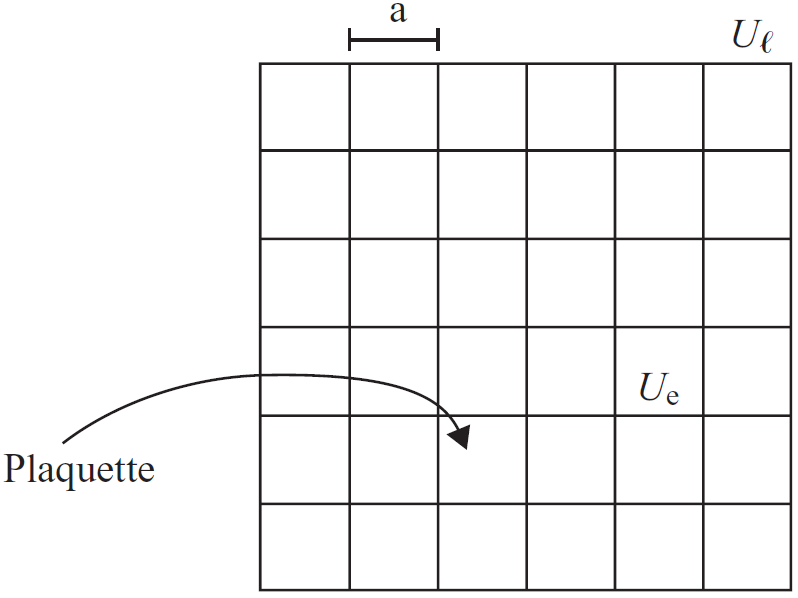
\includegraphics[width=\linewidth]{4.1}}
            \end{minipage}
            \begin{minipage}{0.61\linewidth}
                \vtop{\begin{itemize}{\leftmargin=0em \itemindent=0em}
                    \item<2-> Fix a cubic lattice with $N$ vertices connected by edges of length $a$ in spacetime.
                    \item<3-> Associate an element $U_\mathtt{e}\in\mathbf{SU}(2)$ with each oriented edge $\mathtt{e}$.
                    \item<4-> $U_\mathtt{e}^{-1}$ represents the same edge with the opposite orientation.
                \end{itemize}}
            \end{minipage}
        \end{figure*}\FloatBarrier
        \item<5-> The set of group elements $U_\mathtt{e}$, for all edges of the lattice, provides a natural discretization of the continuous field $A$.
    \end{list}
\end{frame}

\begin{frame}{Lattice gauge theories}
    \begin{list}{\,}{\leftmargin=1em \itemindent=0em}
        \item<1-> The path ordered exponential of a connection $A$ in a group $G$ on a manifold along a path $\gamma$ is called \textit{holonomy}, given by,
        \begin{equation}
            U_\gamma=\operatorname{P}e^{\int_\gamma A}\,,
        \end{equation}
        i.e. $U_\gamma$ is the solution at $s=1$ of the initial value problem,
        \begin{align}
            \dv{s}U(s)=\dv{\gamma^a(s)}{s}A_a(\gamma(s))\,,\,\,\,\,\,\,\,\,\,\,\,\,\,\, U(0)=\mathbb{I}\,.
        \end{align}
        \item<2-> $U_\gamma$ is invariant under local gauge transformations $A\to A+\text{D}\gamma$ everywhere except at the boundary points of $\gamma$.
        \item<3-> The group element $U_\mathtt{e}$ is a holonomy of connection $A$ along edge $\mathtt{e}$,
        \begin{equation}
            U_\mathtt{e}=\operatorname{P}e^{\int_\mathtt{e} A}\,.
        \end{equation}
        \item<4-> Truncating the continuous $\mathbf{SU}(2)$ Yang–Mills theory to group variables $U_\mathtt{e}$ reduces the local $\mathbf{SU}(2)$ gauge symmetry to that at the vertices $\mathtt{v}$ only, with the gauge group of the lattice theory  becoming ${\mathbf{SU}(2)}^N$.
    \end{list}
\end{frame}

\begin{frame}{Lattice gauge theories}
    \begin{list}{\,}{\leftmargin=1em \itemindent=0em}
        \item<1-> Under such gauge transformations, the group variables transform as,
        \begin{equation}
            U_\mathtt{e}\to\lambda_{s_\mathtt{e}}\,U_\mathtt{e}\,\lambda_{t_\mathtt{e}}^{-1}\,,\,\,\,\,\,\,\, \lambda_{\mathtt{v}}\in\mathbf{SU}(2)\,,
        \end{equation}
        where $s_\mathtt{e}$ and $t_\mathtt{e}$ are respectively, the \textit{source} and \textit{target} vertices of $\mathtt{e}$.
        \item<2-> Discrete version of curvature is given by ordered product of four group elements around an elementary square in the lattice (or \textit{plaquette}) $\mathtt{f}$,
        \begin{equation}\label{u_f}
            U_\mathtt{f}=U_\mathtt{e_1}U_\mathtt{e_2}U_\mathtt{e_3}U_\mathtt{e_4}\,.
        \end{equation}
        Its trace is gauge invariant.
        \item<3-> For small $a$, the continuous action is approximated by discrete action,
        \begin{equation}
            S[U]=\beta\sum_\mathtt{f}\mathbf{Tr}U_\mathtt{f}+\text{c.c.}\,\,,
        \end{equation}
        where the coupling constant $\beta$ is such that $\beta\to 0$ as $a\to 0$.
    \end{list}
\end{frame}

\begin{frame}{Lattice gauge theories}
    \begin{list}{\,}{\leftmargin=1em \itemindent=0em}
        \item<1-> For fixed values of boundary edges (or \textit{links}) $\ell$, integrating exponential of action over bulk group elements, we obtain the transition amplitude of the truncated theory,
        \begin{equation}
            W(U_\ell)=\int\dd{U_\mathtt{e}}e^{\frac{i}{\hbar}S[U]}.
        \end{equation}
        Continuum transition amplitudes are recovered in $\beta\to 0,N\to\infty$ limit. Boundary vertices are called \textit{nodes} ($\mathtt{n}$).
        \item<2-> Group elements $U_\ell$ on the boundary edges form the configuration space coordinates with conjugate momentum $L^i_\ell$ for each link $\ell$.
        \item<3-> The corresponding Poisson brackets are (no summation over $\ell$),
        \begin{align}
            \{U_\ell\,,U_{\ell'}\}&=0\,,\\
            \{U_{\ell}\,,L^i_{\ell'}\}&=\delta_{\ell\ell'}\,U_\ell\,\tau^i\,,\\
            \{L^i_{\ell}\,,L^j_{\ell'}\}&=\delta_{\ell\ell'}\,{\epsilon^{ij}}_k\, L^k_{\ell}\,.
        \end{align}
    \end{list}
\end{frame}

\begin{frame}{Lattice gauge theories}
    \begin{list}{\,}{\leftmargin=1em \itemindent=0em}
        \item<1-> The Hilbert space of states $\psi(U_\ell)$ carries a scalar product, invariant under boundary gauge transformations, given by $\mathbf{SU}(2)$ Haar measure,
        \begin{equation}
            (\phi,\psi)=\int_{\mathbf{SU}(2)}\dd{U_\ell}\,\overline{\phi(U_\ell)}\,\psi(U_\ell)\,.
        \end{equation}
        \item<2-> For a quantum harmonic oscillator $V(q)=\frac{1}{2}\omega^2 q^2$, the functional integral (eq. \ref{functional_int}) is given as a limit of an $\epsilon$-discretization at level $N$,
        \begin{equation}
            W(q_s,t_s,q_t,t_t)=\lim_{N\to\infty}\epsilon^{N/2}\int\dd[N]{q}\,e^{\frac{i}{\hbar}S_N(q_n)}\,,
        \end{equation}
        where $\epsilon=(t_t-t_s)/N$, $\Omega\equiv\epsilon\omega$ and the discretized action is, 
        \begin{equation}
            S_N(q_n)=\sum_{n=1}^N\left(\frac{m(q_{n+1}-q_n)^2}{2}-\frac{\Omega^2}{2}q_n^2\right)\,.
        \end{equation}
        \item<3-> It is of common occurrence in lattice gauge theories that the continuum limit is obtained by increasing the number of lattice sites ($N\to\infty$) while also scaling down lattice spacing ($\epsilon\to 0$), or, equivalently, sending appropriate constant(s) $\Omega$ to their critical value(s) $\Omega_\text{c}$ (here zero).
    \end{list}
\end{frame}

\begin{frame}{Lattice gauge theories}
    \begin{list}{\,}{\leftmargin=1em \itemindent=0em}
        \item<1-> Discretizing the same system after parameterization (eq. \ref{para_cov}),
        \begin{align}
            S&=\int\dd{\tau}\left(\frac{m}{2}\frac{(q')^2}{t'}-t'V(q)\right)\\
            &=\sum_{n=1}^N\epsilon\left(\frac{m}{2}\frac{\frac{(q_{n+1}-q_n)^2}{\epsilon^2}}{\frac{(t_{n+1}-t_n)}{\epsilon}}-\frac{(t_{n+1}-t_n)}{\epsilon}V(q_n)\right)\\
            &=\sum_{n=1}^N\left(\frac{m}{2}\frac{(q_{n+1}-q_n)^2}{(t_{n+1}-t_n)}-(t_{n+1}-t_n)V(q_n)\right)\,.
        \end{align}
        Just as the original action did not depend on the parameterization $\tau$, its discretization does not depend upon the lattice spacing (or $\epsilon$).
        \item<2-> Reparameterization-invariant systems (general covariant theories) only require more number of lattice sites $N$ to get a better approximation, without any other parameter to be tuned (unlike lattice QCD).
        \item<3-> It is a general feature of lattice gauge theories that original invariances are restored in the limit of no discretization.
    \end{list}
\end{frame}

%\subsection{Regge calculus}

\begin{frame}{Regge calculus}
    \begin{list}{\,}{\leftmargin=1em \itemindent=0em}
        \item A $d$-simplex is a generalization of a triangle or tetrahedron to $d$ dimensions. Its $d+1$ vertices are connected by $d(d+1)/2$ line segments whose lengths $L_\mathtt{s}$ fully specify the shape of the simplex.
        \item A Regge manifold $(M,L_\mathtt{s})$ in $d$ dimensions is a $d$-dimensional metric space obtained by gluing $d$-simplices along matching boundary $(d-1)$-simplices. These (oriented) structures are called \textit{triangulations}.\\\noindent\FloatBarrier
        \begin{figure*}[!ht]
            \begin{minipage}{\linewidth}
                \centering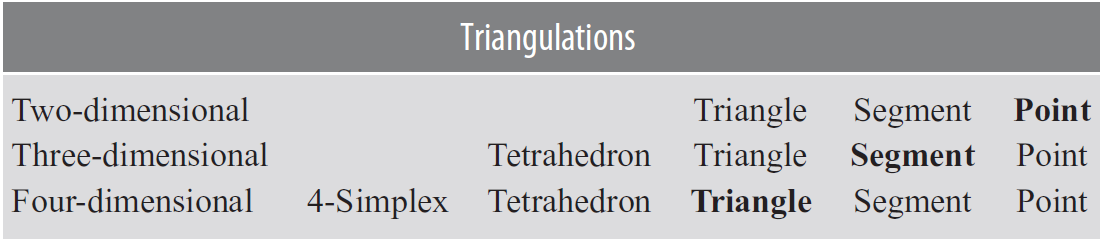
\includegraphics[width=0.8\linewidth]{4.2}
            \end{minipage}
        \end{figure*}\FloatBarrier
        \item In 2D, we obtain a surface by gluing \textit{triangles}, bounded by \textit{segments}, which meet at \textit{points}.
        \item In 3D, we chop space into \textit{tetrahedra}, bounded by triangles, in turn bounded by segments, which meet at points.
        \item In 4D, spacetime is cut into \textit{4-simplices}, bounded by tetrahedra, in turn bounded by triangles, in turn bounded by segments that meet at points.
    \end{list}
\end{frame}

\begin{frame}{Regge calculus}
    \begin{list}{\,}{\leftmargin=1em \itemindent=0em}
        \item A Riemannian manifold $(M,g)$ can be approximated arbitrarily well by a Regge manifold. For any $(M,g)$ and any $\epsilon$, we can find an $(M,L_\mathtt{s})$ such that for any two points in $M$ the difference between their Riemannian distance and the Regge distance is less than $\epsilon$.
        \item Triangulations of $d$-simplices generate curvature on $(d-2)$-simplices, called \textit{hinges} ($\mathtt{h}$).
        \item \noindent\FloatBarrier
        \begin{figure*}[!ht]
            \begin{minipage}{0.3\linewidth}
                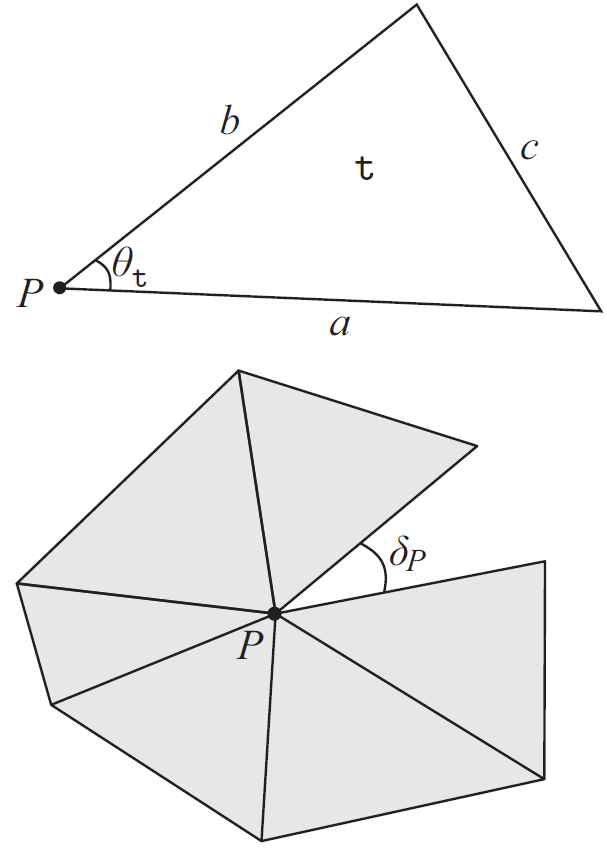
\includegraphics[width=\linewidth]{4.3}
            \end{minipage}
            \begin{minipage}{0.7\linewidth}
                \begin{itemize}{\leftmargin=0em \itemindent=0em}
                    \item In 2D, consider a point $P$ of the triangulation.
                    \item Let angles at $P$ of triangles be $\theta_\mathtt{t}$. We know,
                    \begin{equation}
                        \cos{\theta_\mathtt{t}}=\frac{c^2-a^2-b^2}{2ab}\,.
                    \end{equation}
                    \item If the angles around $P$ sum up to $2\pi$, the manifold is flat at $P$. The Regge curvature at $P$ can be defined as the \textit{deficit angle},
                    \begin{equation}
                        \delta_P(L_\mathtt{s})=2\pi-\sum_\mathtt{t} \theta_\mathtt{t}(L_\mathtt{s})\,.
                    \end{equation}
                \end{itemize}
            \end{minipage}
        \end{figure*}\FloatBarrier
    \end{list}
\end{frame}

\begin{frame}{Regge calculus}
    \begin{list}{\,}{\leftmargin=1em \itemindent=0em}
        \item<1-> \noindent\FloatBarrier
        \begin{figure*}[!ht]
            \begin{minipage}{0.25\linewidth}
                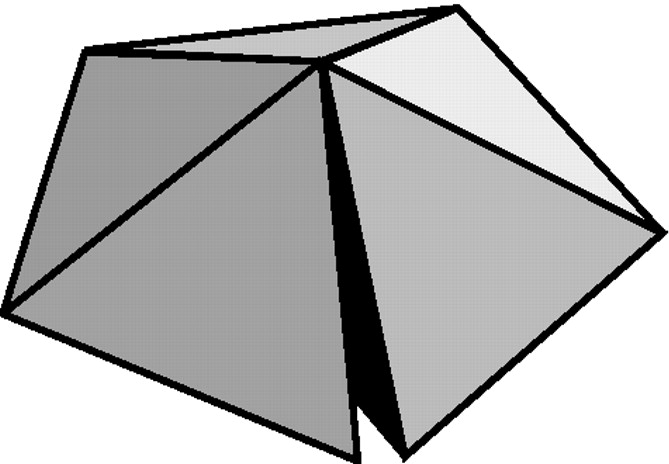
\includegraphics[width=\linewidth]{4.4}
                \caption{}
                \label{fig:4.4}
            \end{minipage}
            \begin{minipage}{0.75\linewidth}
                In higher dimensions, the Regge curvature is still given by a single deficit angle. $P$ is replaced by a $(d-2)$-simplex (a segment in 3D and a triangle in 4D). The sum is over the (pairs of) $(d-1)$-simplices around it (triangles in 3D and tetrahedra in 4D).
            \end{minipage}
        \end{figure*}\FloatBarrier
        \item<2-> \noindent\FloatBarrier
        \begin{figure*}[!ht]
            \begin{minipage}{0.3\linewidth}
                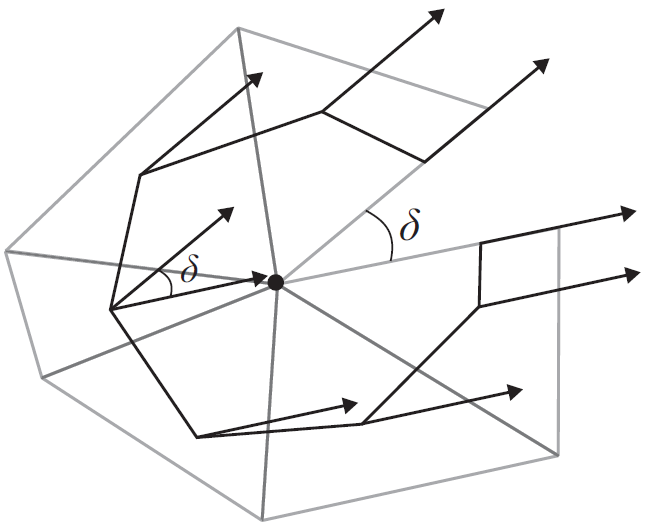
\includegraphics[width=\linewidth]{4.5}
            \end{minipage}
            \begin{minipage}{0.7\linewidth}
                Parallel transport of a vector in a loop around a $(d-2)$-simplex (hinge $\mathtt{h}$) leaves the vector back-rotated by the deficit angle. The Regge action of a Regge manifold $(M,L_\mathtt{s})$ is defined as,
                \begin{equation}
                    S_M(L_\mathtt{s})=\sum_\mathtt{h}A_\mathtt{h}(L_\mathtt{s})\delta_\mathtt{h}(L_\mathtt{s})\,,
                \end{equation}
                where $A_\mathtt{h}$ is the $(d-2)$-volume of $\mathtt{h}$ (length in 3D and area in 4D).
            \end{minipage}
        \end{figure*}\FloatBarrier
        \item<3-> Regge action $S_M(L_\mathtt{s})$ converges to the Einstein–Hilbert action $S[g]$ when the Regge manifold $(M,L_\mathtt{s})$ converges to the Riemannian manifold $(M,g)$, i.e. with sufficiently many simplices/triangulations.
    \end{list}
\end{frame}

%\subsection{Discretization of general relativity}

\begin{frame}{Discretization of general relativity}
    \begin{list}{\,}{\leftmargin=1em \itemindent=0em}
        \item<1-> The Regge discretization is based on metric variables and the segments of the triangulation are subjected to triangle inequalities.
        \item<2-> To obtain a discretization based on the tetrad-connection formalism, we consider the \textit{dual} of a triangulation (in a combinatorial sense). 
        \item<3-> \noindent\FloatBarrier
        \begin{figure*}[!ht]
            \begin{minipage}{0.3\linewidth}
                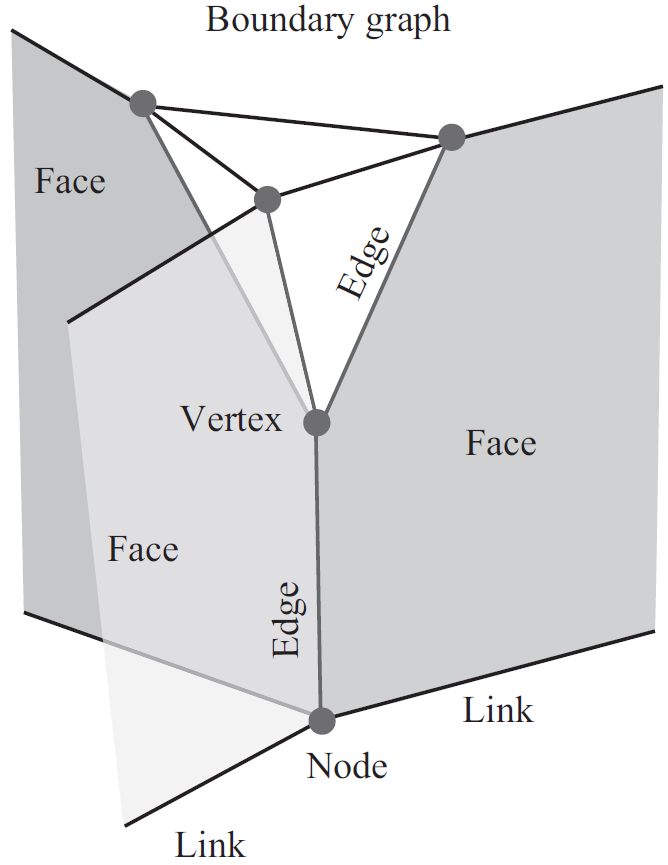
\includegraphics[width=\linewidth]{4.6}
            \end{minipage}
            \begin{minipage}{0.7\linewidth}
                \begin{itemize}{\leftmargin=0em \itemindent=0em}
                    \item<3-> Let $\Delta^\text{*}$ be the dual of a triangulation $\Delta$.
                    \item<4-> A \textit{vertex} $\mathtt{v}$ is dual to a chunk of spacetime (4-simplex $\upsilon$ in 4D and tetrahedron $\uptau$ in 3D).
                    \item<5-> In 3D, an \textit{edge} $\mathtt{e}$ is dual to the triangle $\mathtt{t}$ that separates two tetrahedra. In 4D, it is dual to the tetrahedron between two 4-simplices.
                    \item<6-> A \textit{face} $\mathtt{f}$ is associated to each segment $\mathtt{s}$ of triangulation in 3D and each triangle in 4D.
                    \item<7-> They inherit orientation from their duals in $\Delta$.
                \end{itemize}
            \end{minipage}
        \end{figure*}\FloatBarrier
        \item<8-> The set of vertices, edges and faces is called a \textit{2-complex}, defined by the combinatorial structure of the boundary relations between them.
    \end{list}
\end{frame}

\begin{frame}{Discretization of general relativity}
    \begin{list}{\,}{\leftmargin=1em \itemindent=0em}
        \item<1-> On the boundary, the discretization leads to a graph. The boundary graph $\Gamma$ is both the boundary of the 2-complex $\Delta^\text{*}$ and the dual of the boundary of the triangulation $\Delta$, i.e. $\Gamma=\partial\left(\Delta^\text{*}\right)=\left(\partial\Delta\right)^\text{*}$.
        \item<2-> A boundary vertex (or \textit{node} $\mathtt{n}$) is dual to a chunk of space (tetrahedron in 4D and triangle in 3D). A boundary edge (or \textit{link} $\ell$) is dual to triangles of boundary triangulation in 4D and segments in 3D.\FloatBarrier
        \begin{figure*}[!ht]
            \begin{minipage}{0.56375\linewidth}
                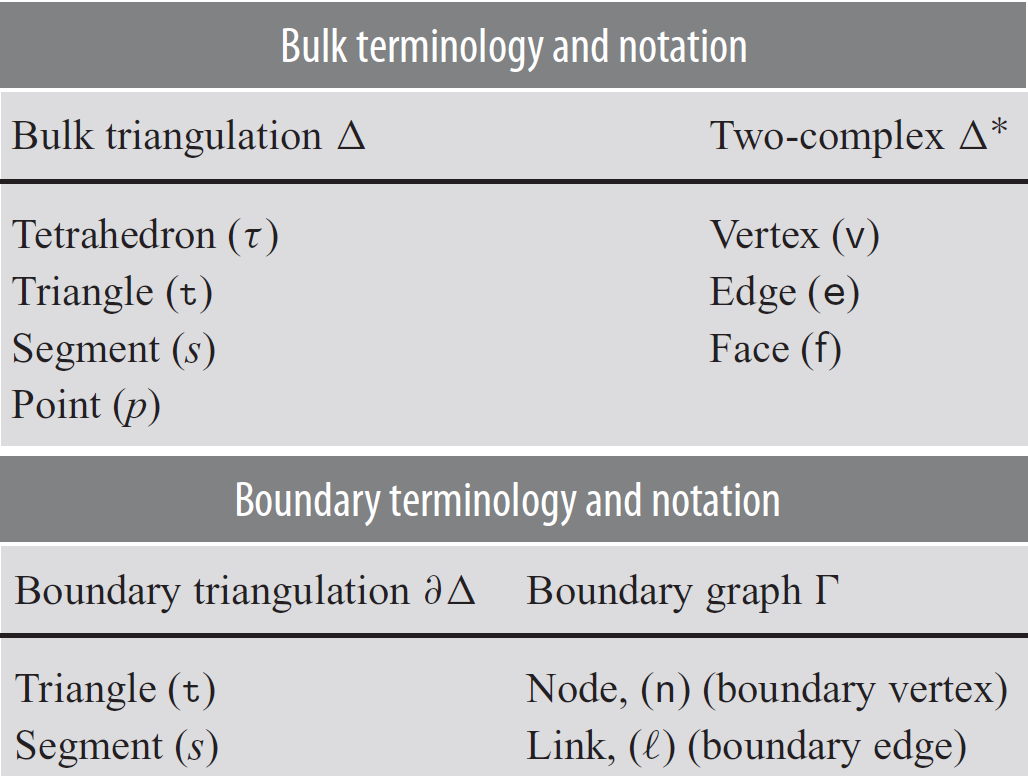
\includegraphics[width=\linewidth]{4.7}
                \caption{In 3D}
            \end{minipage}
            \begin{minipage}{0.43625\linewidth}
                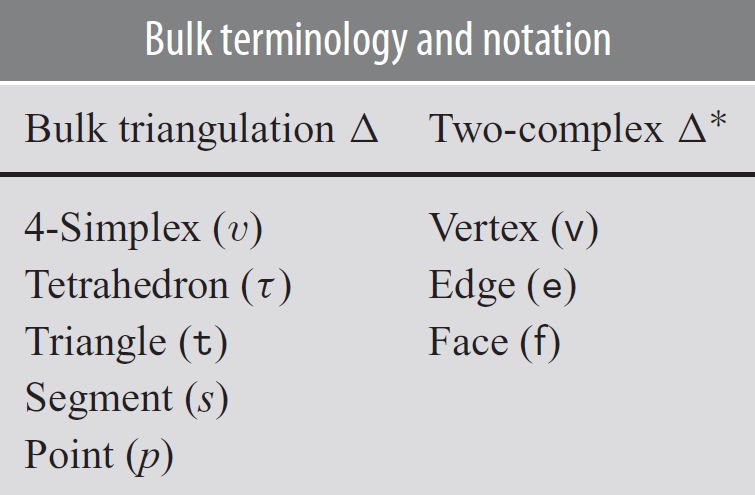
\includegraphics[width=\linewidth]{4.8}
                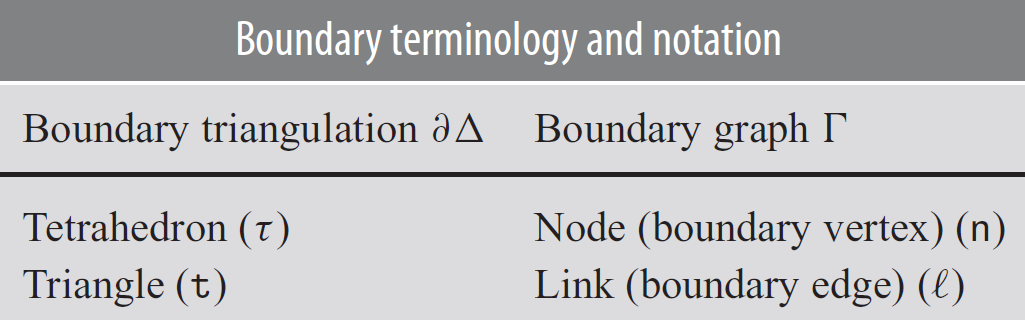
\includegraphics[width=\linewidth]{4.9}
                \caption{In 4D}
            \end{minipage}
        \end{figure*}\FloatBarrier
    \end{list}
\end{frame}

\begin{frame}{Discretization of general relativity}
    \FloatBarrier
    \begin{figure*}[!ht]
        \begin{minipage}{0.5\linewidth}
            \vtop{\centering{In 3D}
            \begin{itemize}
                \item<1-> The connection is discretized by assigning $U_\mathtt{e}\in\mathbf{SU}(2)$ to each edge $\mathtt{e}$ of $\Delta^\text{*}$.
                \begin{equation}
                    \omega\to U_\mathtt{e}=\operatorname{P} e^{\int_\mathtt{e} \omega}\in\mathbf{SU}(2)\,.
                \end{equation}
                \item<2-> The triad is discretized by assigning $L_\mathtt{s}^i\in\mathbb{R}^3$ to each segment $\mathtt{s}$ of $\Delta$.
                \begin{equation}
                    e\to L_\mathtt{s}^i=\int_\mathtt{s}e^i\in\mathbb{R}^3\,.
                \end{equation}
            \end{itemize}}
        \end{minipage}
        \begin{minipage}{0.5\linewidth}
            \vtop{\centering{In 4D}
            \begin{itemize}
                \item<1-> The connection is discretized by assigning $U_\mathtt{e}\in\mathbf{SL}(2,\mathbb{C})$ to each edge $\mathtt{e}$ of $\Delta^\text{*}$.
                \begin{equation}
                    \omega\to U_\mathtt{e}=\operatorname{P} e^{\int_\mathtt{e} \omega}\in\mathbf{SL}(2,\mathbb{C})\,.
                \end{equation}
                \item<2-> The tetrad is discretized by assigning $B_\mathtt{f}\in\mathfrak{sl}(2,\mathbb{C})$ to each triangle $\mathtt{t}$ of $\Delta$ (or face $\mathtt{f}$ of $\Delta^\text{*}$).
                \begin{equation}
                    e\to B_\mathtt{f}=\int_\mathtt{t_f} B\in\mathfrak{sl}(2,\mathbb{C})\,.
                \end{equation}
            \end{itemize}}
        \end{minipage}
    \end{figure*}\FloatBarrier
    \begin{list}{\,}{\leftmargin=1em \itemindent=0em}
        \item<3-> Group variables $U$ transform ``well'' under corresponding gauge transformations. Hence, in the discrete theory the local gauge invariance is reduced to transformations at vertices. It is not so for the algebra variables $L$ and $B$, unless a suitable gauge is chosen.
    \end{list}
\end{frame}

\begin{frame}{Discretization of general relativity}
    \begin{list}{\,}{\leftmargin=1em \itemindent=0em}
        \item<1-> Just like the 4D case, in 3D too the algebra variable $L_\mathtt{s}^i$ can be assigned to a face $\mathtt{f}$ of $\Delta^\text{*}$, the one dual to the segment $\mathtt{s}=\mathtt{s_f}$, i.e. $L_\mathtt{f}^i=L_\mathtt{s_f}^i$.
        \item<2-> The variable $L_\mathtt{f}^i$ can be expressed as an element of the $\mathfrak{su}(2)$ algebra,
        \begin{equation}
            L_\mathtt{f}=L_\mathtt{f}^i \tau_i \in\mathfrak{su}(2)\,.
        \end{equation}
        \item<3-> \noindent\FloatBarrier
        \begin{figure*}[!ht]
            \begin{minipage}{0.35\linewidth}
                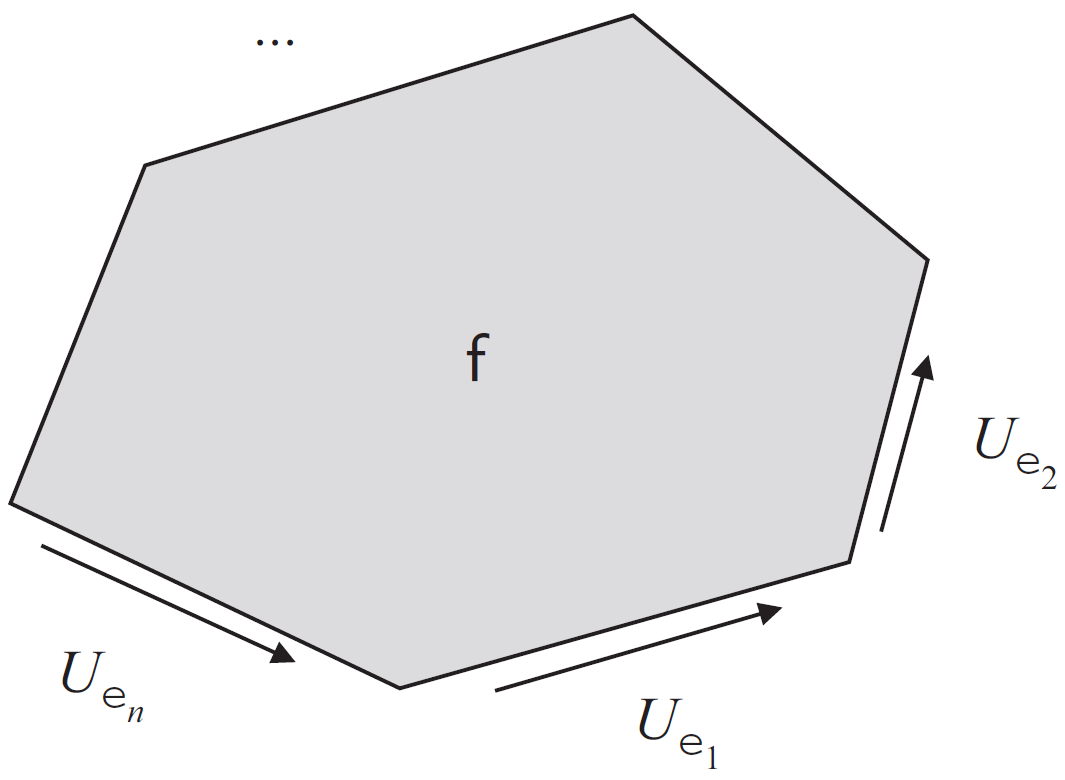
\includegraphics[width=\linewidth]{4.10}
            \end{minipage}
            \begin{minipage}{0.65\linewidth}
                Analogous to eq. \ref{u_f}, we can associate a single group element $U_\mathtt{f}$ with a face $\mathtt{f}$ bounded by edges $\mathtt{e}_1,\dots,\mathtt{e}_n$,
                \begin{equation}
                    U_\mathtt{f}=U_{\mathtt{e}_1}\cdots U_{\mathtt{e}_n}\,.
                \end{equation}
                $U_\mathtt{f}=\mathbb{I}$ implies flatness.
            \end{minipage}
        \end{figure*}\FloatBarrier
        \item<4-> In 3D, the discretized action becomes,
        \begin{equation}
            S=\frac{1}{8\pi G}\sum_\mathtt{f} \mathbf{Tr}(L_\mathtt{f} U_\mathtt{f})\,.
        \end{equation}
        Variation of $L_\mathtt{f}$ in $S$ gives $U_\mathtt{f}=\mathbb{I}$, equivalent to continuous vacuum Einstein field equations in 3D.
    \end{list}
\end{frame}

%\section{3D Euclidean theory}

%\subsection{Quantum kinematics - Hilbert space}

\begin{frame}{Quantum kinematics - Hilbert space}
    \begin{list}{\,}{\leftmargin=1em \itemindent=0em}
        \item<1-> There is one boundary segment $\mathtt{s}$ for each link $\ell$ of the boundary graph $\Gamma$. Thus, at the boundary, the algebra variable $L_\mathtt{s}$ can be renamed as $L_\ell$.
        \item<2-> The Poisson brackets of the discrete boundary phase space are the same (up to $8\pi G$) as those for the $\mathbf{SU}(2)$ Yang–Mills theory on the lattice,
        \begin{align}
            \{U_\ell\,,U_{\ell'}\}&=0\,,\\
            \{U_{\ell}\,,L^i_{\ell'}\}&=(8\pi G)\, \delta_{\ell\ell'}\,U_\ell\,\tau^i\,,\\
            \{L^i_{\ell}\,,L^j_{\ell'}\}&=(8\pi G)\, \delta_{\ell\ell'}\,{\epsilon^{ij}}_k\, L^k_{\ell}\,.
        \end{align}
        \item<3-> We seek operators $\hat{U}_\ell$ and $\hat{L}^i_\ell$ that realize relations such as,
        \begin{equation}\label{3d_comm}
            [\hat{U}_{\ell}\,,\hat{L}^i_{\ell'}]=i\,(8\pi\hbar G)\, \delta_{\ell\ell'}\,\hat{U}_\ell\,\tau^i\,.
        \end{equation}
        \item<4-> Corresponding to a boundary graph $\Gamma$ with $L$ links, the Hilbert space is the space of square integrable functions of the \textit{coordinates} $U_\ell$,
        \begin{equation}
            \mathcal{H}_\Gamma=L^2[{\mathbf{SU}(2)}^L]\,.
        \end{equation}
    \end{list}
\end{frame}

\begin{frame}{Quantum kinematics - Hilbert space}
    \begin{list}{\,}{\leftmargin=1em \itemindent=0em}
        \item<1-> As before, the Hilbert space of states $\psi(U_\ell)$ carries a scalar product, given by $\mathbf{SU}(2)$ invariant Haar measure $\dd{U}$,
        \begin{equation}
            \braket{\psi}{\phi}=\int_{{\mathbf{SU}(2)}^L}\dd{U_\ell} \,\overline{\psi(U_\ell)}\,\phi(U_\ell)\,.
        \end{equation}
        \item<2-> The self-adjoint $\mathbf{SU}(2)$-covariant derivative operator on functions $\psi(U_\ell)$ is the left invariant vector field $\vec{J}$,
        \begin{equation}
            \left(\hat{J}^i\psi\right)(U)\equiv-i\left.\dv{t}\psi(Ue^{t\tau_i})\right\rvert_{t=0}\,.
        \end{equation}
        \item<3-> With $\hat{U}_{\ell}$ as a multiplicative operator, triad operator satisfying eq. \ref{3d_comm} is,
        \begin{equation}
            \vec{L}_\ell\equiv(8\pi\hbar G)\,\vec{J}_\ell\,.
        \end{equation}
        \item<4-> Since $\vec{J}$ is a generator of $\mathbf{SU}(2)$, the length of boundary segment is,
        \begin{align}
            L_{j_{\ell}}&=8\pi\hbar G \sqrt{j_{\ell}(j_{\ell}+1)}\,, &j_{\ell}&=0,\frac{1}{2},1,\frac{3}{2},2,\dots \,\,.
        \end{align}
        Length is quantized.
    \end{list}
\end{frame}

\begin{frame}{Spin networks}
    \begin{list}{\,}{\leftmargin=1em \itemindent=0em}
        \item<1-> To fully define the boundary Hilbert space we must ensure the theory is invariant under $\mathbf{SU}(2)$ gauge transformations. Particularly,
        \begin{equation}
            \psi(U_\ell)=\psi(\Lambda_{s_\ell}U_\ell\Lambda_{t_\ell}^{-1})\,,\,\,\,\,\,\,\, \Lambda_{\mathtt{n}}\in\mathbf{SU}(2)\,.
        \end{equation}
        \item<2-> Equivalently, this relation can be expressed for every node $\mathtt{n}$ of the boundary graph $\Gamma$ (with links $\ell_1,\ell_2,\ell_3$ emerging from it) as,
        \begin{equation}\label{gauss_const_3d}
            \vec{C}_\mathtt{n}\,\psi=(\vec{L}_{\ell_1}+\vec{L}_{\ell_2}+\vec{L}_{\ell_3})\,\psi=0\,,
        \end{equation}
        where $\vec{C}_\mathtt{n}$ is an $\mathbf{SU}(2)$ generator. This is known as the \textit{Gauss constraint}.\\
        It implies that the triangle bounded by segments dual to $\ell_1,\ell_2,\ell_3$ closes.
        \item<3-> For $L$ links and $N$ nodes of $\Gamma$, the subspace of $\mathcal{H}_\Gamma$ where eq. \ref{gauss_const_3d} holds is,
        \begin{equation}
            \mathcal{K}_\Gamma=L^2[{\mathbf{SU}(2)}^L/\,{\mathbf{SU}(2)}^N]_\Gamma\,.
        \end{equation}
        \item<4-> We choose a basis of the eigenvectors $\ket{j_\ell}$ of length operators $L_\ell$. Spin $j_\ell$ is assigned to each link $\ell$ of the boundary graph $\Gamma$ called a \textbf{spin network}.
    \end{list}
\end{frame}

\begin{frame}{Spin networks}
    \begin{list}{\,}{\leftmargin=1em \itemindent=0em}
        \item<1-> As functions of $\mathbf{SU}(2)$, Wigner matrices $D^j(U)$ form an orthogonal basis,
        \begin{equation}
            \int\dd{U}\overline{D^{j'}_{m'n'}(U)}D^{j}_{mn}(U)=\frac{1}{(2j+1)}\, \delta^{jj'}\delta_{mm'}\delta_{nn'}\,.
        \end{equation}
        Hilbert space $L^2[{\mathbf{SU}(2)}]$ can be decomposed into a direct sum of finite dimensional subspaces of spin $j$.
        \item<2-> $D^j(U)$ maps Hilbert space $\mathcal{H}_j$ of the spin $j$ representation to itself. Thus,
        \begin{equation}
            L^2[{\mathbf{SU}(2)}]=\oplus_j(\mathcal{H}_j\otimes\mathcal{H}_j)\,.
        \end{equation}
        \item<3-> The boundary state space of the theory has the structure,
        \begin{equation}
            L^2[{\mathbf{SU}(2)}^L]=\otimes_\ell\left[\oplus_j(\mathcal{H}_j\otimes\mathcal{H}_j)\right]=\oplus_{j_\ell}\otimes_\ell(\mathcal{H}_j\otimes\mathcal{H}_j)\,.
        \end{equation}
        The two Hilbert spaces associated with a link belong to its two ends.
    \end{list}
\end{frame}

\begin{frame}{Spin networks}
    \begin{list}{\,}{\leftmargin=1em \itemindent=0em}
        \item<1-> \noindent\FloatBarrier
        \begin{figure*}[!ht]
            \begin{minipage}{0.15\linewidth}
                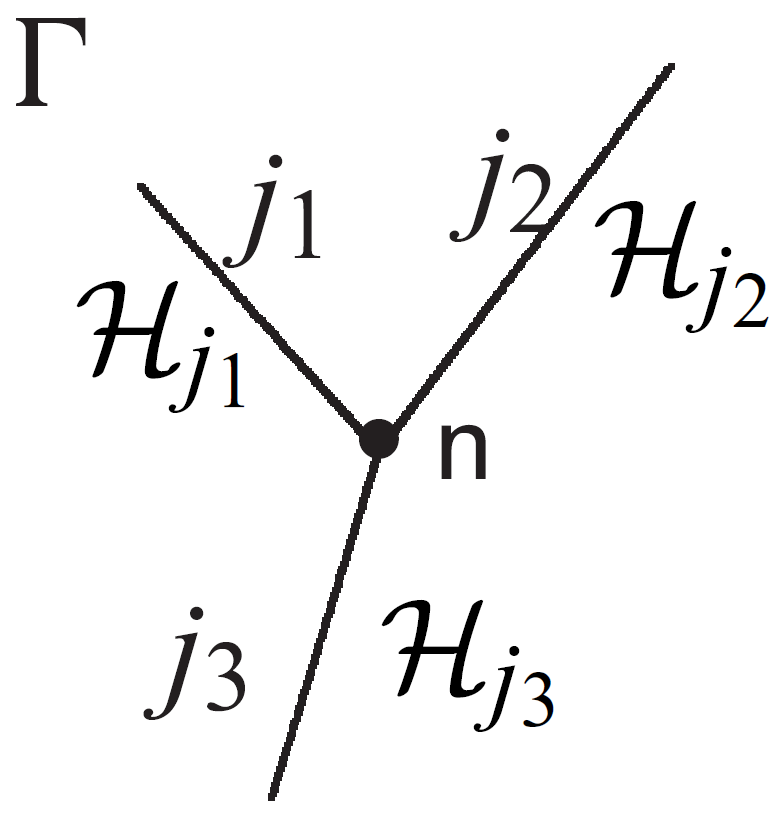
\includegraphics[width=\linewidth]{4.11}
            \end{minipage}
            \begin{minipage}{0.85\linewidth}
                With spins $j_1,j_2,j_3$ coming out from node $\mathtt{n}$, grouping together the Hilbert spaces next to the same node, we have,
                \begin{equation}
                    L^2[{\mathbf{SU}(2)}^L]=\oplus_{j_\ell}\otimes_\mathtt{n}(\mathcal{H}_{j_1}\otimes\mathcal{H}_{j_2}\otimes\mathcal{H}_{j_3})\,.
                \end{equation}
            \end{minipage}
        \end{figure*}\FloatBarrier
        \item<2-> Restricting to the invariant subspace,
        \begin{equation}
            L^2[{\mathbf{SU}(2)}^L/\,{\mathbf{SU}(2)}^N]=\oplus_{j_\ell}\otimes_\mathtt{n}\mathbf{Inv}_{\mathbf{SU}(2)}(\mathcal{H}_{j_1}\otimes\mathcal{H}_{j_2}\otimes\mathcal{H}_{j_3})\,,
        \end{equation}
        which requires,
        \begin{align}
            \lvert j_1-j_2\rvert<&j_3<j_1+j_2\,,&\text{and}\,,& &j_1+j_2+j_3&\in\mathbb{Z}\,. 
        \end{align}
        Spins are the lengths of the sides of the triangle surrounding the node. Hence, these relations imply that they satisfy the triangular inequalities.
        \item<3-> If the above relations hold the invariant space is one-dimensional,
        \begin{equation}
            \mathbf{Inv}_{\mathbf{SU}(2)}(\mathcal{H}_{j_1}\otimes\mathcal{H}_{j_2}\otimes\mathcal{H}_{j_3})=\mathbb{C}\,.
        \end{equation}
        \item<4-> Therefore, restricting to the $j_\ell$ that satisfy the above relations, we get,
        \begin{equation}
            L^2[{\mathbf{SU}(2)}^L/\,{\mathbf{SU}(2)}^N]=\oplus_{j_\ell}\mathbb{C}\,.
        \end{equation}
    \end{list}
\end{frame}

\begin{frame}{Spin networks}
    \begin{list}{\,}{\leftmargin=1em \itemindent=0em}
        \item<1-> A generic quantum state in loop quantum gravity is a superposition of the spin-network states,
        \begin{equation}
            \ket{\psi}=\sum_{j_\ell}\mathcal{C}_{j_\ell}\ket{\,{j_\ell}}\,.
        \end{equation}
        \item<2-> The spin-network wavefunctions are expressed as,
        \begin{equation}
            \psi_{j_\ell}(U_\ell)=\braket{U_\ell}{\,j_\ell}\,.
        \end{equation}
        \item<3-> A state $\psi(U)$ can be written in the Wigner-matrix basis,
        \begin{equation}
            \psi(U)=\sum_{jmn}\mathcal{C}_{jmn}D^j_{mn}(U)\,.
        \end{equation}
        \item<4-> Since states in this theory are functions of $L$ group elements, we write,
        \begin{equation}
            \psi(U_\ell)=\sum_{\substack{j_1\dots j_L \\ m_1\dots m_L \\ n_1\dots n_L}}\mathcal{C}_{j_1\dots j_L m_1\dots m_L n_1\dots n_L} D^{j_1}_{m_1n_1}(U_{\ell_1})\cdots D^{j_L}_{m_Ln_L}(U_{\ell_L})\,.
        \end{equation} 
    \end{list}
\end{frame}

\begin{frame}{Spin networks}
    \begin{list}{\,}{\leftmargin=1em \itemindent=0em}
        \item<1-> Due to $\mathbf{SU}(2)$ gauge-invariance at the nodes, the boundary state must be invariant under transformations of the three group elements of the three links that meet at the node. The only invariant object with three indices in $\mathbf{SU}(2)$ representations is the Wigner 3-$j$ symbol, written as,
        \begin{equation}
            \iota^{m_1m_2m_3}=
            \begin{pmatrix}
                j_1 & j_2 & j_3 \\
                m_1 & m_2 & m_3
            \end{pmatrix}\,.
        \end{equation}
        The Wigner 3-$j$ symbols are also called the trivalent \textit{intertwiners}.
        \item<2-> Any invariant state in the theory is proportional to the normalized state,
        \begin{equation}
            \ket{i}=\sum_{m_1m_2m_3}
            \begin{pmatrix}
                j_1 & j_2 & j_3 \\
                m_1 & m_2 & m_3
            \end{pmatrix}
            \ket{j_1,m_1}\otimes\ket{j_2,m_2}\otimes\ket{j_3,m_3}\,.
        \end{equation}
        \item<3-> With one matrix $D$ for each link $\ell$ and one 3-$j$ symbol $\iota$ for each node $\mathtt{n}$, the gauge-invariant states have the form,
        \begin{equation}
            \psi(U_\ell)=\sum_{j_1\dots j_L}\mathcal{C}_{j_1\dots j_L}\iota^{m_1m_2m_3}_1\cdots\iota^{m_{L-2}m_{L-1}m_L}_N D^{j_1}_{m_1n_1}(U_{\ell_1})\cdots D^{j_L}_{m_Ln_L}(U_{\ell_L})\,.
        \end{equation} 
    \end{list}
\end{frame}

\begin{frame}{Spin networks}
    \begin{list}{\,}{\leftmargin=1em \itemindent=0em}
        \item<1-> A generic gauge-invariant state is a linear combination,
        \begin{equation}
            \psi(U_\ell)=\sum_{j_\ell}\mathcal{C}_{j_\ell}\psi_{j_\ell}(U_\ell)\,,
        \end{equation}
        of the orthogonal states,
        \begin{equation}
            \psi_{j_\ell}(U_\ell)=\iota^{m_1m_2m_3}_1\cdots\iota^{m_{L-2}m_{L-1}m_L}_N D^{j_1}_{m_1n_1}(U_{\ell_1})\cdots D^{j_L}_{m_Ln_L}(U_{\ell_L})\,,
        \end{equation}
        labelled by a spin associated with each link.
        \item<2-> The spin-network wavefunctions can be concisely written as,
        \begin{equation}
            \psi_{j_\ell}(U_\ell)=\braket{U_\ell}{j_\ell}=\bigotimes_\mathtt{n}\iota_\mathtt{n}\cdot\,\bigotimes_\ell D^{j_\ell}(U_\ell)\,.
        \end{equation}
        These are the three-dimensional spin-network states in the group representation.
    \end{list}
\end{frame}

%\subsection{Quantum dynamics - transition amplitudes}

\begin{frame}{Quantum dynamics - transition amplitudes}
    \begin{list}{\,}{\leftmargin=1em \itemindent=0em}
        \item<1-> The transition amplitude is a function of states defined on the boundary graph $\Gamma=\left(\partial\Delta\right)^\text{*}$ of a triangulation $\Delta$ of spacetime,
        \begin{align}
            W_\Delta(U_\ell)&=\braket{W_\Delta}{U_\ell}\,, &W_\Delta(j_\ell)&=\braket{W_\Delta}{\,j_\ell}\,.
        \end{align}
        \item<2-> The transition amplitude $W_\Delta$ of the discretized theory is given using the Feynman path integral, ($\mathcal{N}$ is a normalization factor),
        \begin{align}
            W_\Delta(U_\ell)&=\mathcal{N}\int\dd{U_\mathtt{e}}\int\dd{L_\mathtt{f}}e^{\frac{i}{8\pi\hbar G}\sum_\mathtt{f}\mathbf{Tr}(L_\mathtt{f} U_\mathtt{f})}\,\\
            &=\mathcal{N}\int\dd{U_\mathtt{e}}\prod_\mathtt{f}\delta(U_\mathtt{f})\,.
        \end{align}
        \item<3-> The delta function can be expanded over $\mathbf{SU}(2)$ representations,
        \begin{equation}
            \delta(U)=\sum_j(2j+1)\mathbf{Tr}D^{j}(U)\,.
        \end{equation}
        $\mathbf{Tr}D^{j}(U)$ is the character of the representation of dimension $2j+1$.
    \end{list}
\end{frame}

\begin{frame}{Quantum dynamics - transition amplitudes}
    \begin{list}{\,}{\leftmargin=1em \itemindent=0em}
        \item<1-> Since $U_\mathtt{f}$ is the product of group elements associated with the links $1\mathtt{f},\dots,n\mathtt{f}$ around the face $\mathtt{f}$ (with associated spin $j_\mathtt{f}$),
        \begin{align}
            W_\Delta(U_\ell)&=\mathcal{N}\int\dd{U_\mathtt{e}}\prod_\mathtt{f}\sum_j(2j+1)\mathbf{Tr}D^{j}(U_\mathtt{f})\,\\
            &=\mathcal{N}\,\sum_{j_\mathtt{f}}\left(\prod_\mathtt{f}(2j_\mathtt{f}+1)\right)\int\dd{U_\mathtt{e}}\prod_\mathtt{f}\mathbf{Tr}\left(D^{j_\mathtt{f}}(U_{1\mathtt{f}})\cdots D^{j_\mathtt{f}}(U_{n\mathtt{f}})\right)\,.
        \end{align}
        \item<2-> Each edge $\mathtt{e}$ is dual to a triangle, bounded by three segments, in turn dual to three faces. Therefore, each $\dd{U_\mathtt{e}}$ integral is of the form,
        \begin{equation}
            \int\dd{U}D^{j_{\ell_1}}_{m_1n_1}(U)D^{j_{\ell_2}}_{m_2n_2}(U)D^{j_{\ell_3}}_{m_3n_3}(U)\,.
        \end{equation}
        \item<3-> Following similar arguments as earlier, normalization is given by,
        \begin{align}
            \int\dd{U}D^{j_{1}}_{m_1n_1}(U)D^{j_{2}}_{m_2n_2}(U)D^{j_{3}}_{m_3n_3}(U)&=\iota^{m_1m_2m_3}\iota^{n_1n_2n_3} \\ &=
            \begin{pmatrix}
                j_1 & j_2 & j_3 \\
                m_1 & m_2 & m_3
            \end{pmatrix}
            \begin{pmatrix}
                j_1 & j_2 & j_3 \\
                n_1 & n_2 & n_3
            \end{pmatrix}\,.
        \end{align}
    \end{list}
\end{frame}

\begin{frame}{Quantum dynamics - transition amplitudes}
    \begin{list}{\,}{\leftmargin=1em \itemindent=0em}
        \vspace{-2pt}
        \item<1-> Since there are four edges at each vertex (in 3D), there are four 3-$j$ symbols, each contracted using $g_{mn}$ to raise/lower magnetic indices,
        \begin{equation}
            g_{mn}=\sqrt{2j+1}
            \begin{pmatrix}
                j & j & 0 \\
                m & n & 0
            \end{pmatrix}
            =(-1)^{j-m}\,\delta_{m,-n}\,.
        \end{equation}
        \vspace{-7pt}
        \item<2-> $\mathbf{SU}(2)$ invariant contraction of four 3-$j$ symbols gives Wigner 6-$j$ symbol,
        \begin{align}
            \begin{Bmatrix}
                j_1 & j_2 & j_3 \\
                j_4 & j_5 & j_6
            \end{Bmatrix}
            \equiv\sum_{m_a,n_a}\prod_{a=1}^{6} g_{m_an_a}&
            \begin{pmatrix}
                j_1 & j_2 & j_3 \\
                m_1 & m_2 & m_3
            \end{pmatrix}
            \begin{pmatrix}
                j_1 & j_4 & j_5 \\
                n_1 & m_4 & m_5
            \end{pmatrix}\notag\\
            \times&
            \begin{pmatrix}
                j_2 & j_4 & j_6 \\
                n_2 & n_4 & m_6
            \end{pmatrix}
            \begin{pmatrix}
                j_3 & j_5 & j_6 \\
                n_3 & n_5 & n_6
            \end{pmatrix}\,.
        \end{align}
        \vspace{-6pt}
        \item<3-> With $M=\sum_{a=1}^{6}m_a$ and $J=\sum_{a=1}^{6}j_a$,
        \vspace{-3pt}
        \begin{align}
            \begin{Bmatrix}
                j_1 & j_2 & j_3 \\
                j_4 & j_5 & j_6
            \end{Bmatrix}
            &=\,(-1)^{J-M}\,\sum_{m_a}
            \begin{pmatrix}
                j_1 & j_2 & j_3 \\
                m_1 & m_2 & m_3
            \end{pmatrix}
            \begin{pmatrix}
                j_1 & j_4 & j_5 \\
                -m_1 & m_4 & m_5
            \end{pmatrix}\notag\\
            &\times
            \begin{pmatrix}
                j_2 & j_4 & j_6 \\
                -m_2 & -m_4 & m_6
            \end{pmatrix}
            \begin{pmatrix}
                j_3 & j_5 & j_6 \\
                -m_3 & -m_5 & -m_6
            \end{pmatrix}\,.
        \end{align}
    \end{list}
\end{frame}

\begin{frame}{Quantum dynamics - transition amplitudes}
    \begin{list}{\,}{\leftmargin=1em \itemindent=0em}
        \item<1-> Integrating over internal-edge variables, we get (in spin representation),
        \begin{equation}\label{ponz_reg}
            W_\Delta(j_\ell)=\mathcal{N}_\Delta\sum_{j_\mathtt{f}}\,\prod_\mathtt{f}(-1)^{j_\mathtt{f}}(2j_\mathtt{f}+1)\,\prod_\mathtt{v}(-1)^{J_\mathtt{v}}\{6\text{-}j\}\,,
        \end{equation}
        where $J_\mathtt{v}=\sum_{a=1}^{6}j_a$ and $j_a$ are spins of the faces adjacent to vertex $\mathtt{v}$.
        \item<2-> The transition amplitude so obtained is characterized by the properties:
        \begin{itemize}
            \item<2-> \textit{Superposition principle}: Amplitudes are given by the sum of elementary amplitudes (Feynman's sum over paths $\sigma$),
            \vspace{-1pt}
            \begin{equation}
                \braket{W}{\psi}=\sum_\sigma W(\sigma)\,.
            \end{equation}
            \item<3-> \vspace{-2pt}\textit{Locality}: Elementary amplitudes can be expressed as products of amplitudes associated with spacetime points (or vertices $\mathtt{v}$),
            \vspace{-1pt}
            \begin{equation}
                W(\sigma)\sim\prod_\mathtt{v}W_\mathtt{v}\,.
            \end{equation}
            \item<4-> \vspace{-2pt}\textit{Local Euclidean invariance}: Vertex amplitude (namely $\{6\text{-}j\}$) can be expressed as projection on $\mathbf{SU}(2)$ invariant part of the state $\psi_\mathtt{v}$,
            \vspace{-1pt}
            \begin{equation}
                W_\mathtt{v}=(\operatorname{P_{\mathbf{SU}(2)}}\psi_\mathtt{v})(\mathbb{I})\,.
            \end{equation}
        \end{itemize}
    \end{list}
\end{frame}

\begin{frame}{Ponzano–Regge model}
    Ponzano and Regge obtained eq. \ref{ponz_reg}, and developed the following model.
    \begin{list}{\,}{\leftmargin=1em \itemindent=0em}
        \item<1-> Consider a tetrahedron of volume $V$ determined by the lengths of its six sides $L_1,\dots,L_6$, with associated spins $j_1,\dots,j_6$ such that $L_a=j_a+\frac{1}{2}$.
        \item<2-> With Regge action $S$, in the limit of large $j$'s (classical limit),\vspace{-3pt}
        \begin{equation}
            \{6\text{-}j\}\,\opsim\limits_{j\to\infty}\,\frac{1}{\sqrt{12\pi V}}\cos{\left(S+\frac{\pi}{4}\right)}\,,
        \end{equation}
        \begin{equation}
            \text{or,\,\,\,\,\,\,\,\,\,\,\,\,\,\,\,\,\,}\{6\text{-}j\}\,\opsim\limits_{j\to\infty}\,\frac{1}{2\sqrt{-12i\pi V}}e^{iS}+\frac{1}{2\sqrt{12i\pi V}}e^{-iS}\,.
        \end{equation}
        \item<3-> Eq. \ref{ponz_reg} defines a discretization of the path-integral of quantum gravity,\vspace{-3pt}
        \begin{equation}
            Z\sim\int\mathcal{D}[g]\,e^{\frac{i}{\hbar}\int\sqrt{-g}R}\,.
        \end{equation}
        \item<4-> Obtaining the continuum limit by refining the triangulation $\Delta$, keeping the boundary graph fixed,\vspace{-4pt}
        \begin{equation}
            W=\lim_{p\to\infty}\,\lim_{\Lambda\to\infty}\left(\frac{w}{\Lambda}\right)^p\sum_{j_\mathtt{f}=0}^\Lambda\,\prod_\mathtt{f}(-1)^{j_\mathtt{f}}(2j_\mathtt{f}+1)\,\prod_\mathtt{v}(-1)^{J_\mathtt{v}}\{6\text{-}j\}\,,
        \end{equation}
        where $w$ is a number, $p$ is the number of points in $\Delta$, $\Lambda$ is a spin cut-off.
    \end{list}
\end{frame}

\begin{frame}{Alternative form of the transition amplitude}
    \begin{list}{\,}{\leftmargin=1em \itemindent=0em}
        \item<1-> The partition function of a triangulation $\Delta$ without boundaries is,
        \begin{equation}
            Z=\int\dd{U_\mathtt{e}}\prod_\mathtt{f}\delta(U_{\mathtt{e}_1}\cdots U_{\mathtt{e}_n})\,.
        \end{equation}
        \item<2-> \noindent\FloatBarrier
        \begin{figure*}[!ht]
            \begin{minipage}{0.25\linewidth}
                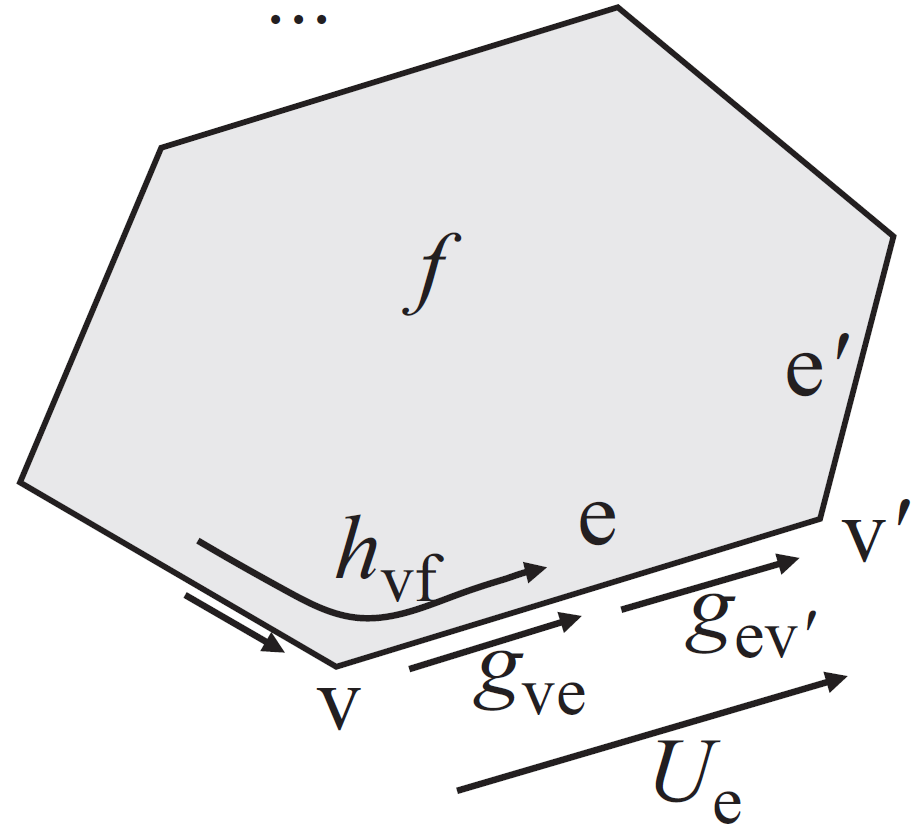
\includegraphics[width=\linewidth]{4.12}
            \end{minipage}
            \begin{minipage}{0.75\linewidth}
                Introducing two variables per link $\ell$, associated with each vertex-edge couple, such that $U_\mathtt{e}=g_{\mathtt{ve}}g_{\mathtt{ev'}}$ and $g_{\mathtt{ve}}=g^{-1}_{\mathtt{ev}}$, we can write,
                \begin{equation}
                    Z=\int\dd{g_\mathtt{ve}}\prod_\mathtt{f}\delta(g_\mathtt{ve}g_\mathtt{ev'}g_\mathtt{v'e'}g_\mathtt{e'v''}\cdots)\,.
                \end{equation}
            \end{minipage}
        \end{figure*}\FloatBarrier
        \item<3-> For vertex $\mathtt{v}$ bounding edges $\mathtt{e}$ and $\mathtt{e'}$ and face $\mathtt{f}$, using $h_\mathtt{vf}=g_{\mathtt{ev}}g_{\mathtt{ve'}}$ ,
        \begin{align}
            Z&=\int\dd{h_\mathtt{vf}}\dd{g_\mathtt{ve}}\prod_\mathtt{f}\delta(g_\mathtt{ve}g_\mathtt{ev'}g_\mathtt{v'e'}g_\mathtt{e'v''}\cdots)\prod_\mathtt{vf}\delta(g_\mathtt{e'v}g_\mathtt{ve}h_\mathtt{vf})\,\\
            &=\int\dd{h_\mathtt{vf}}\dd{g_\mathtt{ve}}\prod_\mathtt{f}\delta(h_\mathtt{vf}h_\mathtt{v'f}\cdots)\prod_\mathtt{vf}\delta(g_\mathtt{e'v}g_\mathtt{ve}h_\mathtt{vf})\,.
        \end{align}
    \end{list}
\end{frame}

\begin{frame}{Alternative form of the transition amplitude}
    \begin{list}{\,}{\leftmargin=1em \itemindent=0em}
        \item<1-> The transition amplitude can be written as,\vspace{-4pt}
        \begin{equation}
            W(h_\ell)=\int\dd{h_\mathtt{vf}}\prod_\mathtt{f}\delta(h_\mathtt{f})\prod_\mathtt{v}A_\mathtt{v}(h_\mathtt{vf})\,,
        \end{equation}
        where $h_\mathtt{f}=\prod\limits_{\mathtt{v}\in\partial\mathtt{f}}h_\mathtt{vf}$ for internal faces and $h_\mathtt{f}=\left(\prod\limits_{\mathtt{v}\in\partial\mathtt{f}}h_\mathtt{vf}\right)h_\ell$ for a face bounded by a link $\ell$, and the vertex amplitude is,\vspace{-4pt}
        \begin{equation}
            A_\mathtt{v}(h_\mathtt{vf})=\mathcal{N}\int\dd{g_\mathtt{ve}}\prod_\mathtt{f}\delta(g_\mathtt{e'v}g_\mathtt{ve}h_\mathtt{vf})\,.
        \end{equation}
        \item<2-> In the vertex amplitude with one group element for each of the $n=4$ edges coming out of a vertex, integration over $n-1$ variables leaves the result invariable under the last integration. Dropping one integration,\vspace{-3pt}
        \begin{equation}
            \int_{{\mathbf{SU}(2)}^n}\dd{g'_{\mathtt{ve}}}\equiv\int_{{\mathbf{SU}(2)}^{n-1}}\dd{g_{\mathtt{ve_1}}}\cdots\dd{g_{\mathtt{ve_{n-1}}}}\,.
        \end{equation}
        \item<3-> Expanding the delta function over $\mathbf{SU}(2)$ representations gives,\vspace{-4pt}
        \begin{equation}
            A_\mathtt{v}(h_\mathtt{vf})=\mathcal{N}\,\sum_{j_\mathtt{f}}\int\dd{g'_\mathtt{ve}}\prod_\mathtt{f}(2j_\mathtt{f}+1)\mathbf{Tr}_{j_\mathtt{f}}[g_\mathtt{e'v}g_\mathtt{ve}h_\mathtt{vf}]\,.
        \end{equation}
    \end{list}
\end{frame}

%\section{4D Lorentzian theory}

%\subsection{Quantum states of gravity}

\begin{frame}{Quantum states of gravity}
    \begin{list}{\,}{\leftmargin=1em \itemindent=0em}
        \item<1-> In the time gauge ($e^0=\dd{t}$, $e^i=e^i_a\dd{x^a}$), the algebra variables on the boundary reduce to,
        \begin{align}
            L^i_\mathtt{f}&=\frac{1}{2\gamma}{\epsilon^{i}}_{jk}\int_{\mathtt{t_\mathtt{f}}}e^j\wedge e^k\,, & \lvert L_\mathtt{f} \rvert =\frac{1}{\gamma} A_{\mathtt{t_\mathtt{f}}}\,,
        \end{align}
        where $A_{\mathtt{t_\mathtt{f}}}$ is the area of the triangle $\mathtt{t_\mathtt{f}}$ lying on the boundary, dual to the face $\mathtt{f}$ bounded by the link $\ell$. Vector $\vec{L}_\mathtt{f}$ is normal to triangle $\mathtt{t_\mathtt{f}}$.
        \item<2-> As in 3D, for each link $\ell$ of the boundary graph $\Gamma$, the boundary variables $U_\ell\in\mathbf{SL}(2,\mathbb{C})$ and $B_\ell\in\mathfrak{sl}(2,\mathbb{C})$ become operators.
        \item<3-> Quantization leads to functions $\psi(U_\ell)$ on ${\mathbf{SL}(2,\mathbb{C})}^L$, where the operator $B_\ell$ is realized as the generator of $\mathbf{SL}(2,\mathbb{C})$ transformations.
        \item<4-> In the classical limit, the components of the generators $B_\ell$ of $\mathbf{SL}(2,\mathbb{C})$ must satisfy the linear simplicity constraint (eq. \ref{linear_simp_const}), $\vec{K}=\gamma\vec{L}$ .
    \end{list}
\end{frame}

\begin{frame}{Quantum states of gravity}
    \begin{list}{\,}{\leftmargin=1em \itemindent=0em}
        \item<1-> The irreducible unitary representations of $\mathbf{SL}(2,\mathbb{C})$ are labelled by a positive real number $p$ and a non-negative half-integer $k$.
        \item<2-> The Hilbert space $V^{(p,k)}$ of the $(p,k)$ representation decomposes into irreducibles of the subgroup $\mathbf{SU}(2)\leq\mathbf{SL}(2,\mathbb{C})$ as,
        \begin{equation}
            V^{(p,k)}=\bigoplus^\infty_{j=k}\mathcal{H}_j\,,
        \end{equation}
        where $\mathcal{H}_j$ is a $2j+1$ dimensional space with spin $j$ irrep of $\mathbf{SU}(2)$.
        \item<3-> Choosing a basis of states $\ket{p,k;j,m}$, with $j=k,k+1,\dots$ and $m=-j,\dots,j$, we have for quantum numbers $j$ of $\lvert\vec{L}\rvert^2$ and $m$ of $L_z$,
        \begin{align}
            \lvert\vec{K}\rvert^2-\lvert\vec{L}\rvert^2 &= p^2-k^2+1\,, &\vec{K}\cdot\vec{L}=pk\,.
        \end{align}
        \item<4-> In the limit of large quantum numbers (classical limit), we must have,
        \begin{align}
            \lvert\vec{K}\rvert^2-\lvert\vec{L}\rvert^2 &= (\gamma^2-1) \lvert\vec{L}\rvert^2 \,, &\vec{K}\cdot\vec{L}=\gamma \lvert\vec{L}\rvert^2\,,
        \end{align}
        or,
        \begin{align}
            p^2-k^2+1 &=(\gamma^2-1)j(j+1)\,, &pk=\gamma j(j+1)\,.
        \end{align}
    \end{list}
\end{frame}

\begin{frame}{Quantum states of gravity}
    \begin{list}{\,}{\leftmargin=1em \itemindent=0em}
        \item<1-> For large quantum numbers, this gives,
        \begin{align}
            p^2-k^2 &=(\gamma^2-1)j^2\,, &pk=\gamma j^2\,.
        \end{align}
        with a solution,
        \begin{align}
            p &=\gamma k\,, & k=j\,.
        \end{align}
        The first relation restricts the set of unitary representations, while the second picks out the lowest spin subspace within each representation.
        \item<2-> The states therefore have the form,
        \begin{equation}
            \ket{p,k;j,m}=\ket{\gamma j,j;j,m}\,.
        \end{equation}
        \item<3-> The states are in one-to-one correspondence with the states in the representations of $\mathbf{SU}(2)$. Hence, we introduce a map $Y_\gamma$ ,
        \begin{align}
            Y_\gamma:\mathcal{H}_j &\to V^{(p=\gamma j,\,k=j)}\,,
            &\ket{j;m}&\mapsto \ket{\gamma j,j;j,m}\,.
        \end{align}
        \item<4-> All vectors in the image of this map satisfy the linear simplicity constraint in the large $j$ limit, i.e. $\mel{Y_\gamma \psi}{\vec{K}-\gamma\vec{L}}{Y_\gamma \phi}=0$.
    \end{list}
\end{frame}

\begin{frame}{Quantum states of gravity}
    \begin{list}{\,}{\leftmargin=1em \itemindent=0em}
        \item<1-> $Y_\gamma$ maps functions over $\mathbf{SU}(2)$ to functions over $\mathbf{SL}(2,\mathbb{C})$,
        \begin{align}
            Y_\gamma:L^2[\mathbf{SU}(2)]&\to F[\mathbf{SL}(2,\mathbb{C})] \,,\\
            \psi(h)= \sum_{jmn}c_{jmn}D^{(j)}_{mn}(h)&\mapsto \psi(g)= \sum_{jmn} c_{jmn}D^{(\gamma j,j)}_{jm,jn}(g)\,.
        \end{align}
        Thus, $Y_\gamma$ maps $\mathbf{SU}(2)$ spin networks to $\mathbf{SL}(2,\mathbb{C})$ spin networks.
        \item<2-> Following the canonical analysis in Ashtekar variables, the generators $\vec{L}_\ell$ of $\mathbf{SU}(2)$ transformations, associated to each link $\ell$ of the boundary graph, are normal to corresponding triangles lying on the boundary of the triangulation with the area given by $A_\ell=8\pi\gamma\hbar G \lvert \vec{L}_\ell \rvert^2$ , or,
        \begin{align}
             A_j&=8\pi\gamma\hbar G\sqrt{j(j+1)}\,, &j=0,\frac{1}{2},1,\frac{3}{2},2,\dots\,\,.
        \end{align}
        \item<3-> For an arbitrary surface punctured by N links,
        \begin{align}
            A_{j_n}&=8\pi\gamma\hbar G\sum_{n=1}^N\sqrt{j_n(j_n+1)}\,, &j_n=0,\frac{1}{2},1,\frac{3}{2},2,\dots\,\,.
        \end{align}
        Hence, we fix the loop quantum gravity length scale $l_o$ by $l_o^2=8\pi\gamma\hbar G$.
    \end{list}
\end{frame}

\begin{frame}{Spin networks in 4D}
    \begin{list}{\,}{\leftmargin=1em \itemindent=0em}
        \item<1-> As in 3D, the Hilbert space is decomposed as,
        \begin{equation}
            L^2[{\mathbf{SU}(2)}^L]=\otimes_\ell\left[\oplus_j(\mathcal{H}_j\otimes\mathcal{H}_j)\right]=\oplus_{j_\ell}\otimes_\ell(\mathcal{H}_j\otimes\mathcal{H}_j)\,,
        \end{equation}
        and,
        \begin{equation}
            L^2[{\mathbf{SU}(2)}^L/\,{\mathbf{SU}(2)}^N]=\oplus_{j_\ell}\otimes_\mathtt{n}\mathbf{Inv}_{\mathbf{SU}(2)}(\mathcal{H}_{j_1}\otimes\mathcal{H}_{j_2}\otimes\mathcal{H}_{j_3}\otimes\mathcal{H}_{j_4})\,,
        \end{equation}
        which differs from the 3D case as each edge dual to a tetrahedron is bounded by four triangles, in turn dual to four faces. Invariant subspace $\mathbf{Inv}_{\mathbf{SU}(2)}(\mathcal{H}_{j_1}\otimes\mathcal{H}_{j_2}\otimes\mathcal{H}_{j_3}\otimes\mathcal{H}_{j_4})$ is not one-dimensional, in general.
        \item<2-> Linearly independent invariant tensors are constructed as,
        \begin{equation}
            \iota^{m_1m_2m_3m_4}_k=
            \begin{pmatrix}
                j_1 & j_2 & k \\
                m_1 & m_2 & m
            \end{pmatrix}
            g_{mn}
            \begin{pmatrix}
                k & j_3 & j_4 \\
                n & m_3 & m_4
            \end{pmatrix}\,,
        \end{equation}
        for any $k$ satisfying,
        \begin{equation}
            \operatorname{max}[\lvert j_1-j_2\rvert,\lvert j_3-j_4\rvert]\geq k\leq\operatorname{min}[j_1+j_2,j_3+j_4]\,.
        \end{equation} 
        These states are denoted by $\ket{k}$.
    \end{list}
\end{frame}

\begin{frame}{Spin networks in 4D}
    \begin{list}{\,}{\leftmargin=1em \itemindent=0em}
        \item<1-> The space $\mathcal{K}_{j_1\dots j_4}=\mathbf{Inv}_{\mathbf{SU}(2)}(\mathcal{H}_{j_1}\otimes\mathcal{H}_{j_2}\otimes\mathcal{H}_{j_3}\otimes\mathcal{H}_{j_4})$ has dimension,
        \begin{equation}
            \operatorname{dim}[\mathcal{K}_{j_1\dots j_4}]=\operatorname{min}[j_1+j_2,j_3+j_4]-\operatorname{max}[\lvert j_1-j_2\rvert,\lvert j_3-j_4\rvert]+1\,.
        \end{equation}
        \item<2-> A generic gauge-invariant state is a linear combination,
        \begin{equation}
            \psi(U_\ell)=\sum_{j_\ell k_\mathtt{n}} \mathcal{C}_{j_\ell k_\mathtt{n}}\psi_{j_\ell k_\mathtt{n}}(U_\ell)\,,
        \end{equation}
        of the orthogonal states,
        \begin{equation}
            \psi_{j_\ell k_\mathtt{n}} (U_\ell)=\iota^{m_1m_2m_3m_4}_{k_1}\cdots\iota^{m_{L-3}m_{L-2}m_{L-1}m_L}_{k_N} D^{j_1}_{m_1n_1}(U_{\ell_1})\cdots D^{j_L}_{m_Ln_L}(U_{\ell_L})\,,
        \end{equation}
        labelled by a spin associated with each link and an \textit{intertwine} quantum number $k$ associated with each node $\mathtt{n}$.
        \item<3-> The spin-network wavefunctions can be concisely written as,
        \begin{equation}
            \psi_{j_\ell k_\mathtt{n}}(U_\ell)= \braket{U_\ell}{j_\ell,k_\mathtt{n}}=\bigotimes_\mathtt{n}\iota_{k_\mathtt{n}}\cdot\,\bigotimes_\ell D^{j_\ell}(U_\ell)\,.
        \end{equation}
        These are the 4D spin-network states in the group representation. 
    \end{list}
\end{frame}

\begin{frame}{Spin networks in 4D}
    \begin{list}{\,}{\leftmargin=1em \itemindent=0em}
        \item<1-> The oriented volume $V$ of a tetrahedron is an observable, given by,
        \begin{equation}
            V^2=\frac{2}{9}\epsilon_{ijk}L^i L^j L^k \,.
        \end{equation}
        \item<2-> In the eigenbasis $\{\ket{\upsilon}\}$ of the volume operator, spin-network states are,
        \begin{equation}
            \psi_{j_\ell \upsilon_\mathtt{n}}(U_\ell)= \braket{U_\ell}{j_\ell,\upsilon_\mathtt{n}}=\bigotimes_\mathtt{n}\iota_{\upsilon_\mathtt{n}}\cdot\,\bigotimes_\ell D^{j_\ell}(U_\ell)\,.
        \end{equation}
        \item<3-> A basis of states in $\mathcal{H}_\Gamma$ is provided by the spin-network states $\ket{\Gamma,j_\ell,\upsilon_\mathtt{n}}$, with a spin $j_\ell$ associated with each link of the graph $\Gamma$ and a volume eigenvalue $\upsilon_\mathtt{n}$ associated with each node $\mathtt{n}$ of the graph $\Gamma$.
        \item<4-> These are eigenstates of the area and volume operators.
        \item<5-> Classically, the residual geometric freedom corresponds to the space of possible shapes of a tetrahedron with fixed volume, bounded by triangles of fixed areas.
    \end{list}
\end{frame}

%\subsection{Transition amplitudes}

\begin{frame}{Transition amplitudes}
    \begin{list}{\,}{\leftmargin=1em \itemindent=0em}
        \item<1-> The form of the transition amplitudes is the same as in 3D,
        \begin{equation}
            W(h_\ell)=\int_{{\mathbf{SU}(2)}}\dd{h_\mathtt{vf}}\prod_\mathtt{f}\delta(h_\mathtt{f})\prod_\mathtt{v}A_\mathtt{v}(h_\mathtt{vf})\,,
        \end{equation}
        but the vertex amplitudes $A_\mathtt{v}(h_\mathtt{vf})$ need to be made $\mathbf{SL}(2,\mathbb{C})$ invariant.
        \item<2-> Using the $Y_\gamma$ map to map functions of $\mathbf{SU}(2)$ variables to functions of $\mathbf{SL}(2,\mathbb{C})$ variables, the vertex amplitude can be expressed as the projection on $\mathbf{SL}(2,\mathbb{C})$ invariant states,
        \begin{equation}
            A_\mathtt{v}(\psi_\mathtt{v})=(\operatorname{P_{\mathbf{SU}(2)}}\circ Y_\gamma\psi_\mathtt{v})(\mathbb{I})\,.
        \end{equation}
        \item<3-> In the group representation,
        \begin{equation}\label{vert_amp_4d}
            A_\mathtt{v}(h_\mathtt{vf})=\mathcal{N}\,\sum_{j_\mathtt{f}}\int_{{\mathbf{SL}(2,\mathbb{C})}}\dd{g'_\mathtt{ve}}\prod_\mathtt{f}(2j_\mathtt{f}+1)\mathbf{Tr}_{j_\mathtt{f}}[Y_\gamma^\dagger g_\mathtt{e'v}g_\mathtt{ve}Y_\gamma h_\mathtt{vf}]\,,
        \end{equation}
        where,
        \begin{equation}
            \mathbf{Tr}_{j_\mathtt{f}}[Y_\gamma^\dagger g Y_\gamma h]=\mathbf{Tr}_{j_\mathtt{f}}[Y_\gamma^\dagger D^{(\gamma j,j)}(g) Y_\gamma D^{(j)}(h)]= \sum_{mn}D^{(\gamma j,j)}_{jm,jn}(g) D^{(j)}_{mn}(h)\,.
        \end{equation}
        The $\mathbf{SL}(2,\mathbb{C})$ integrations are over four out of five group variables.
    \end{list}
\end{frame}

\begin{frame}{Transition amplitudes}
    \begin{list}{\,}{\leftmargin=1em \itemindent=0em}
        \item<1-> The transition amplitude so obtained is characterized by the properties:
        \begin{itemize}
            \item<1-> \textit{Superposition principle}: Amplitudes are given by the sum of elementary amplitudes (Feynman's sum over paths $\sigma$),
            \begin{equation}
                \braket{W}{\psi}=\sum_\sigma W(\sigma)\,.
            \end{equation}
            \item<2-> \textit{Locality}: Elementary amplitudes can be expressed as products of amplitudes associated with spacetime points (or vertices $\mathtt{v}$),
            \begin{equation}
                W(\sigma)\sim\prod_\mathtt{v}W_\mathtt{v}\,.
            \end{equation}
            \item<3-> \textit{Local Euclidean invariance}: The vertex amplitude can be expressed as the projection on $\mathbf{SL}(2,\mathbb{C})$ invariant part of the state $\psi_\mathtt{v}$,
            \begin{equation}
                W_\mathtt{v}=(\operatorname{P_{\mathbf{SL}(2,\mathbb{C})}}\circ Y_\gamma\psi_\mathtt{v})(\mathbb{I})\,.
            \end{equation}
        \end{itemize}
        \item<4-> \vspace{-10pt}Given an observable $\mathcal{O}$, its expectation value is defined as,
        \begin{equation}
            \expval{\mathcal{O}}=\frac{\mel{W}{\mathcal{O}}{\Psi}}{\braket{W}{\Psi}}\,.
        \end{equation}
    \end{list}
\end{frame}

\begin{frame}{Alternative form of transition amplitudes}
    \begin{list}{\,}{\leftmargin=1em \itemindent=0em}
        \item<1-> Performing the $\dd{h_\mathtt{vf}}$ integrals, we obtain,
        \begin{equation}
            W(h_\mathtt{f})=\mathcal{N}\,\sum_{j_\mathtt{f}}\int_{{\mathbf{SL}(2,\mathbb{C})}}\dd{g'_\mathtt{ve}}\mathbf{Tr}_{j_\mathtt{f}}[Y_\gamma^\dagger g_\mathtt{e'v}g_\mathtt{ve}Y_\gamma\cdot Y_\gamma^\dagger g_\mathtt{ev'}g_\mathtt{v'e''}Y_\gamma\cdots]\,.
        \end{equation}
        The trace runs around a face and is called the \textit{face amplitude}.
        \item<2-> \noindent\FloatBarrier
        \begin{figure*}[!ht]
            \begin{minipage}{0.25\linewidth}
                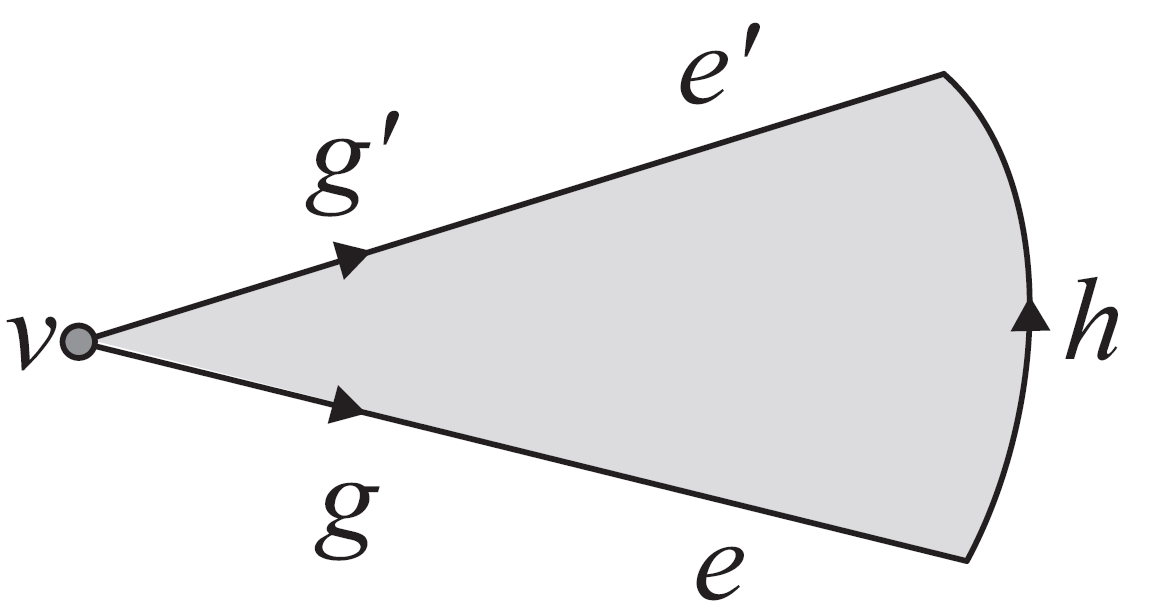
\includegraphics[width=\linewidth]{4.13}
            \end{minipage}
            \begin{minipage}{0.75\linewidth}\centering
                The \textit{wedge amplitude} is defined by,
                \begin{equation}
                    W(g,h)=\sum_j(2j+1)\mathbf{Tr}_{j}[Y_\gamma^\dagger g Y_\gamma h]\,.
                \end{equation}
            \end{minipage}
        \end{figure*}\FloatBarrier
        \item<3-> In the basis of Wigner matrix elements, this becomes,
        \begin{equation}
            W(g,j,m,m')=\mel{j,m'}{Y_\gamma^\dagger g Y_\gamma}{j,m}\,.
        \end{equation}
        \item<4-> As observed by an accelerated observer undergoing a boost ($g=e^{i\eta\mathcal{K}_z}$),
        \begin{equation}
            W_{m,m'}(\eta)=\mel{j,m'}{Y_\gamma^\dagger e^{i\eta\mathcal{K}_z} Y_\gamma}{j,m}\,.
        \end{equation}
    \end{list}
\end{frame}

\begin{frame}{Alternative form of transition amplitudes}
    \begin{list}{\,}{\leftmargin=1em \itemindent=0em}
        \item<1-> In terms of the wedge amplitude, the full amplitude is written as,
        \begin{equation}
            W(h_\ell)=\mathcal{N}\,\int_{{\mathbf{SL}(2,\mathbb{C})}}\dd{h_\mathtt{vf}}\dd{g'_\mathtt{ve}}\prod_{\mathtt{f}}\delta(h_\mathtt{f})\prod_w W(g_\mathtt{e'v}g_\mathtt{ve},h_\mathtt{vf})\,.
        \end{equation}
        \item<2-> It is also convenient to rewrite the vertex amplitude (eq. \ref{vert_amp_4d}) as,
        \begin{equation}
            A_\mathtt{v}(h_\mathtt{vf})=\mathcal{N}\int_{{\mathbf{SL}(2,\mathbb{C})}}\dd{g'_\mathtt{n}}\prod_\ell\operatorname{P}[g_{s(\ell)}g^{-1}_{t(\ell)},h_\ell]\,,
        \end{equation}
        where $\ell,\mathtt{n}$ refer to nodes and links of the vertex graph, and the \textit{kernel},
        \begin{equation}
            \operatorname{P}[g,h]=\sum_j(2j+1)\mathbf{Tr}_{j}[Y_\gamma^\dagger g Y_\gamma h]\,.
        \end{equation}
        \item<3-> Explicitly,
        \begin{equation}
            \operatorname{P}[g,h]=\sum_j(2j+1)\,D^{(\gamma j,j)}_{jm,jn}(g) D^{(j)}_{mn}(h)\,.
        \end{equation}
        This encodes the link between $\mathbf{SU}(2)$ and $\mathbf{SL}(2,\mathbb{C})$.
    \end{list}
\end{frame}

%\section{References}

\begin{frame}{References}
    \begin{list}{\,}{\leftmargin=1em \itemindent=0em}
        \item<1-> The content of this presentation is heavily adapted from - Carlo Rovelli \& Francesca Vidotto. \emph{Covariant Loop Quantum Gravity}. CUP, 2015. Most equations and figures have been taken from the same.
        \item<2-> Top figure on page \pageref{fig:4.4} has been taken from - Conway, J.H. \& Torquato, S. \emph{Packing, tiling, and covering with tetrahedra}. PNAS, July 11, 2006.
    \end{list}
\end{frame}

\end{document}
